\documentclass{beamer}
\usepackage{config}

%Information to be included in the title page:
\title[Github]{Versionner un projet avec Git,\\ Communiquer avec GitHub}
\author{Florian Legendre}
\institute{Université de Poitiers}
\date{Année 2020 - 2021}
\logo{
\includegraphics[scale=0.1]{UP.png}}


%%% ============================================================= %%%
%%% ====================== Début des diapos ===================== %%%
%%% ============================================================= %%%

\begin{document}

\frame{\titlepage}

\begin{frame}
\frametitle{Table of Contents}
\tableofcontents[hideallsubsections]
\end{frame}


%% --------------------- %%
%%        SECTION        %%
%% --------------------- %%
\AtBeginSection[]
{
  \begin{frame}
    \frametitle{Table of Contents}
    \tableofcontents[sectionstyle=show/hide,subsectionstyle=show/show/hide]
  \end{frame}
}


\section{Pourquoi GitHub?}


% Subsection:
\subsection{Les contraintes à respecter}
\begin{frame}{Les contraintes à respecter}
Peu importe la plateforme choisie nous devions respecter les deux contraintes suivantes:
\begin{itemize}
	\item Les données/codes ne doivent pas être accessibles au publique ou à qui que 
	      ce soit d'autres que les personnes autorisées
	\item Les données/codes doivent n'appartenir qu'à vous en tout temps
\end{itemize}
\end{frame}


% Subsection:
\subsection{Un extrait de l'état de l'art}
\begin{frame}{Les autres solutions}

SourceSup RENATER:
% ------------------ Tableau
\tiny
\setlength{\arrayrulewidth}{0.5mm}
\begin{center}
\begin{tabular}{ | m{20em} | m{20em}| } 
\hline
 \rowcolor{lightgray} \multicolumn{2}{|c|}{\textbf{Analyse de la solution SourceSup Renater}} \\
\hline
\cellcolor{green} AVANTAGES & \cellcolor{red} INCONVÉNIENTS \\ 
\hline
\medskip
\begin{itemize}
    \item Service de dépôt distant
    \item Création de forums autour du projet
    \item Documentation du projet par un Wiki / Page web
    \item Serveur de fichiers lourds (300Mo)
    \item Listes de diffusions / Sondages / Abonnements à des forums
    \item Messagerie intégrée
    \item Sécurité des données / Pas de commercialisation des données
    \item Des mots-clés pour les recherches de projets
    \item Extensibilité des services grâce aux plugins
\end{itemize} 

& 
\medskip
\begin{itemize}
    \item Boutons et liens parfois très petits voire illisibles
    \item Style de l'interface un peu vieillissant... Peut ne pas être engageant.
    \item Pas d'intégrations à d'autres plateformes comme Zenado ou Gitter, etc.
    \item Validation des projets déposée un peu floue
    \item Réactivité du support? Survie de la plateforme?
    \item Certaines fonctionnalités peuvent être très techniques
\end{itemize} 
\\ 
\hline
\end{tabular}
\end{center}
\bigskip
\normalsize
% ------------------ Fin Tableau
\end{frame}

\begin{frame}
En-dehors de SourceSup RENATER les solutions étaient soit:

\begin{itemize}
	\item Partielles (GitLab / Bitbucket)
	\item Payantes (Bitbucket)
	\item Les termes d'utilisations étaient flous (GitLab)
	\item Trop techniques à mettre en oeuvre (Allura)
\end{itemize}
\medskip

Si vous voulez tout de même les explorer voici quelques liens:
\begin{itemize}
	\item SourceSup RENATER: \url{https://sourcesup.renater.fr/}
	\item GitLab: \url{https://about.gitlab.com/}
	\item BitBucket: \url{https://bitbucket.org/product/}
	\item Allura: \url{https://allura.apache.org/}
\end{itemize}
\end{frame}


% Subsection:
\subsection{Les motivations de ce choix}
\begin{frame}{Avantages et Inconvénients de GitHub}
% ------------------ Tableau
\setlength{\arrayrulewidth}{0.5mm}
\tiny
\begin{center}
\begin{tabular}{ | m{20em} | m{20em}| } 
\hline
 \rowcolor{lightgray} \multicolumn{2}{|c|}{\textbf{Analyse de GitHub}} \\
\hline
\cellcolor{green} AVANTAGES & \cellcolor{red} INCONVÉNIENTS \\ 
\hline
\medskip
\begin{itemize}
	\item Respect des contraintes énoncées par le biais des projets privés
    \item Nombre de collaborateurs et de projets privés illimité + de nombreux services 
          gratuits (cf. \url{https://github.com/pricing})
    \item Tout-en-un pour la communication/gestion (humaine) des projets 
    \item Possibilité de créer des organisations
    \item La forge n°1 sur le marché => plateforme vivante et dynamique
\end{itemize} 
& 
\medskip
\begin{itemize}
    \item Forge propriétaire (attention à d'éventuels changements des conditions  
          d'utilisation...)
    \item Quelques limitations sur les projets privés avec la formule gratuite 
          (pas de Wiki ni de pages web par exemple)
\end{itemize} 
\\ 
\hline
\end{tabular}
\end{center}
\bigskip
\normalsize
% ------------------ Fin Tableau
\end{frame}




%% --------------------- %%
%%        SECTION        %%
%% --------------------- %%
\AtBeginSection[]
{
  \begin{frame}
    \frametitle{Table of Contents}
    \tableofcontents[sectionstyle=show/hide,subsectionstyle=show/show/hide]
  \end{frame}
}

\section{Communiquer le projet avec GitHub}


% Subsection:
\subsection{Créer un dépôt et régler sa visibilité}
\begin{frame}{Régler la visibilité à la création du dépôt}
\begin{center}
	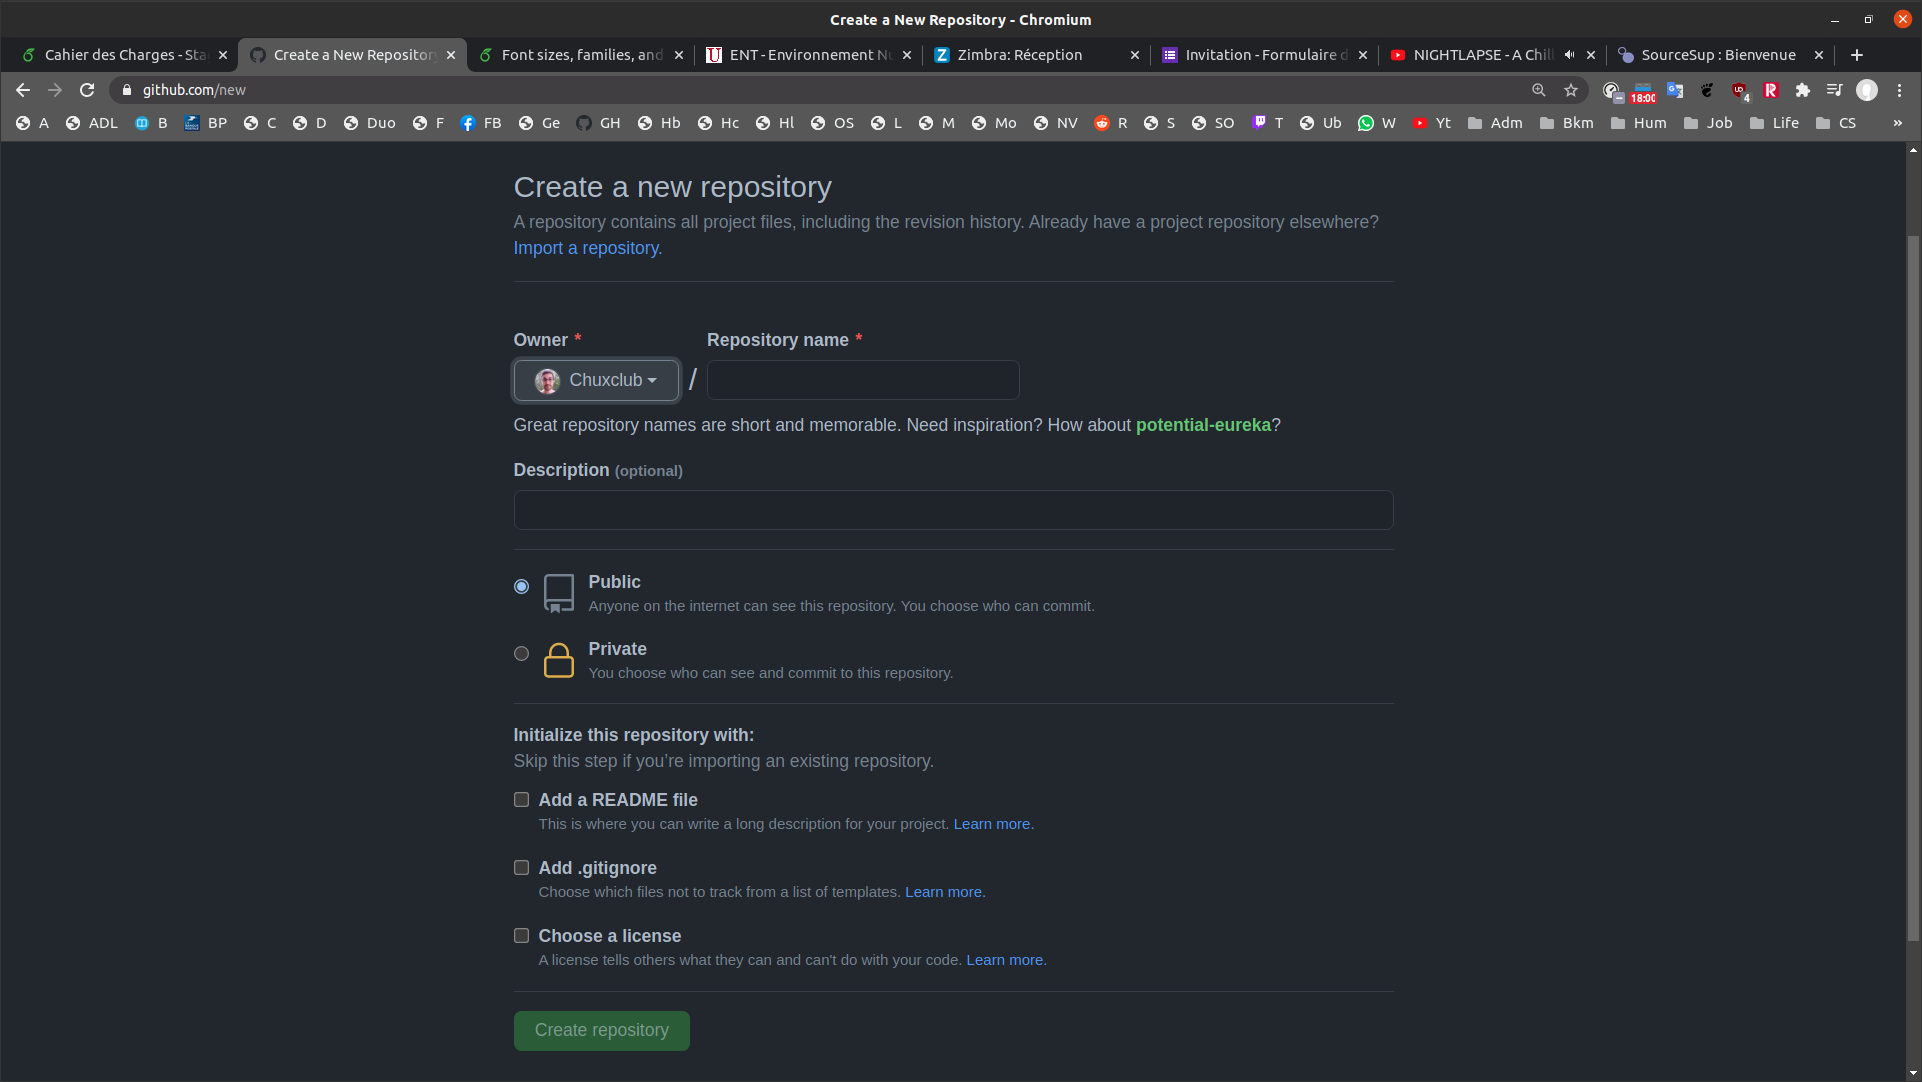
\includegraphics[scale=0.15]{github_createRepo.png}
\end{center}
\end{frame}

\begin{frame}{Régler la visibilité après la création du dépôt}
\begin{center}
	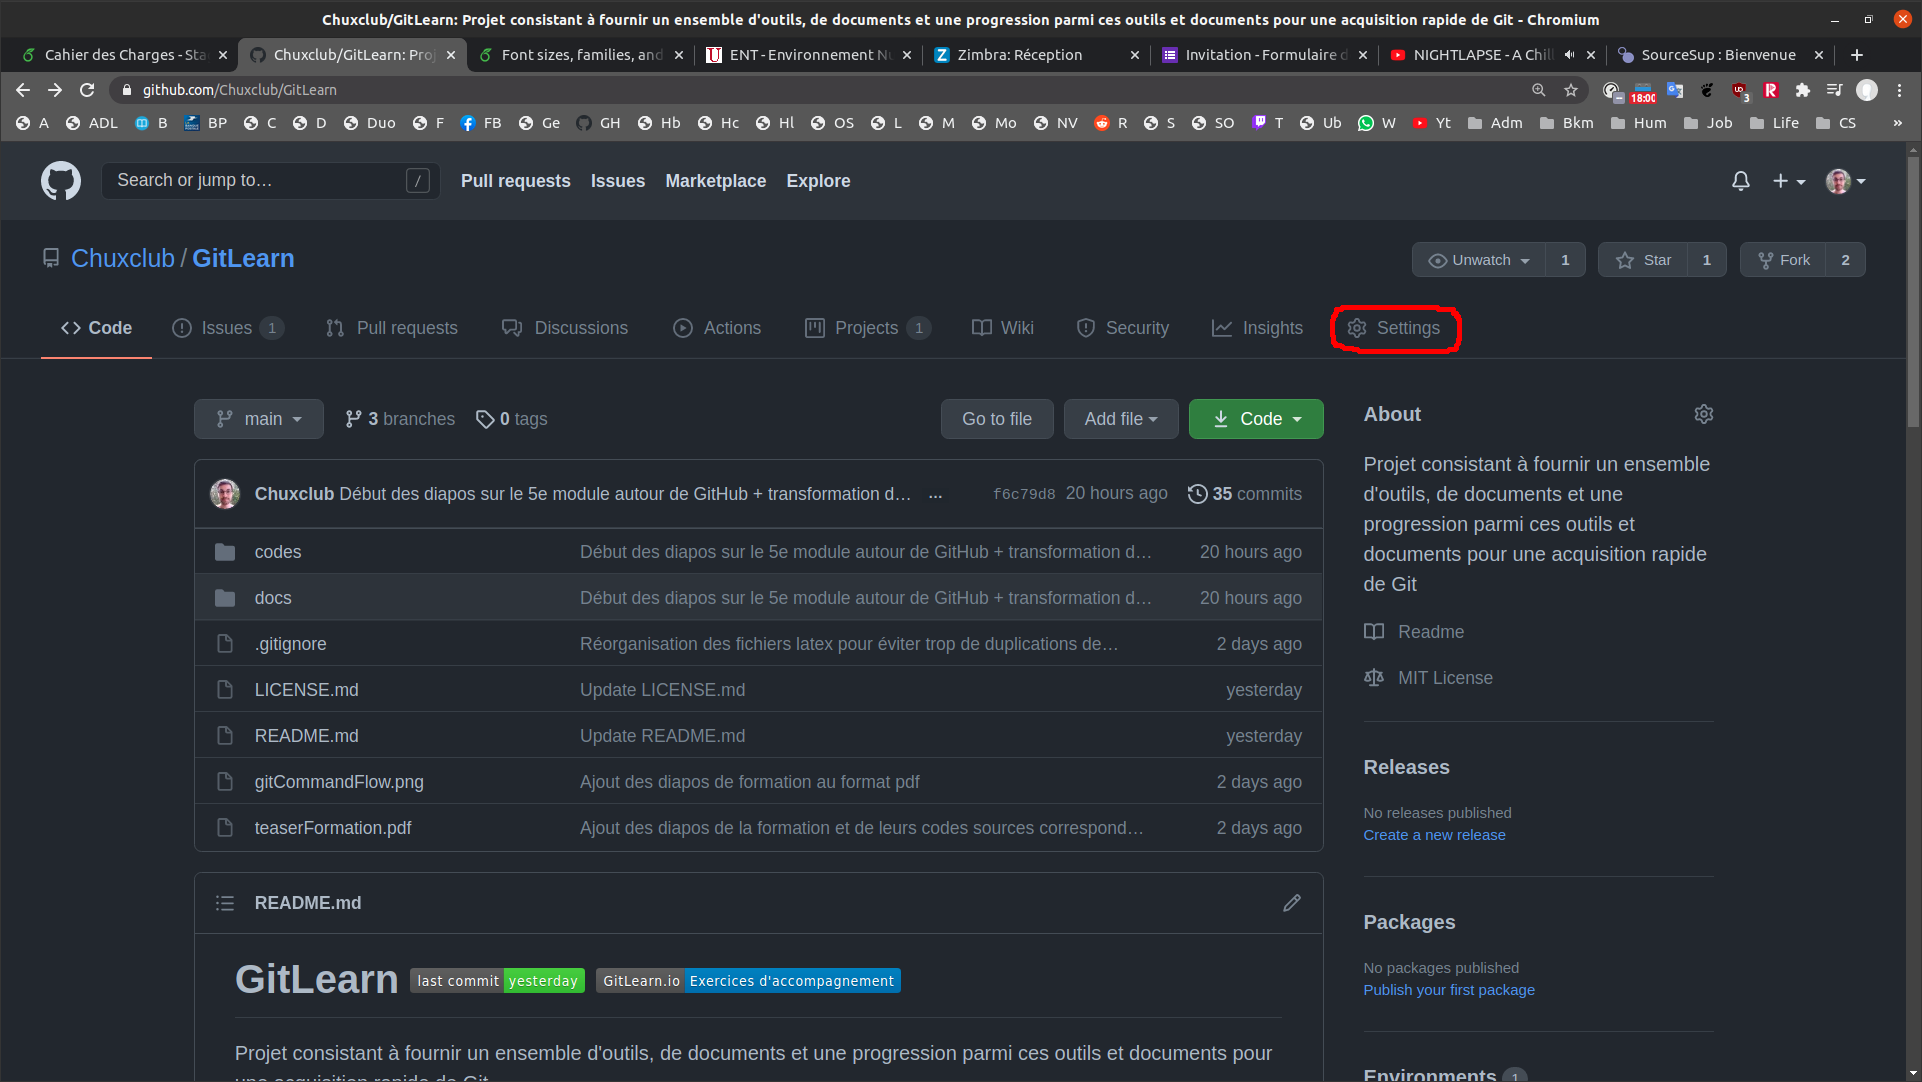
\includegraphics[scale=0.15]{github_settings_E.png}
\end{center}
\end{frame}

\begin{frame}{Régler la visibilité après la création du dépôt}
\begin{center}
	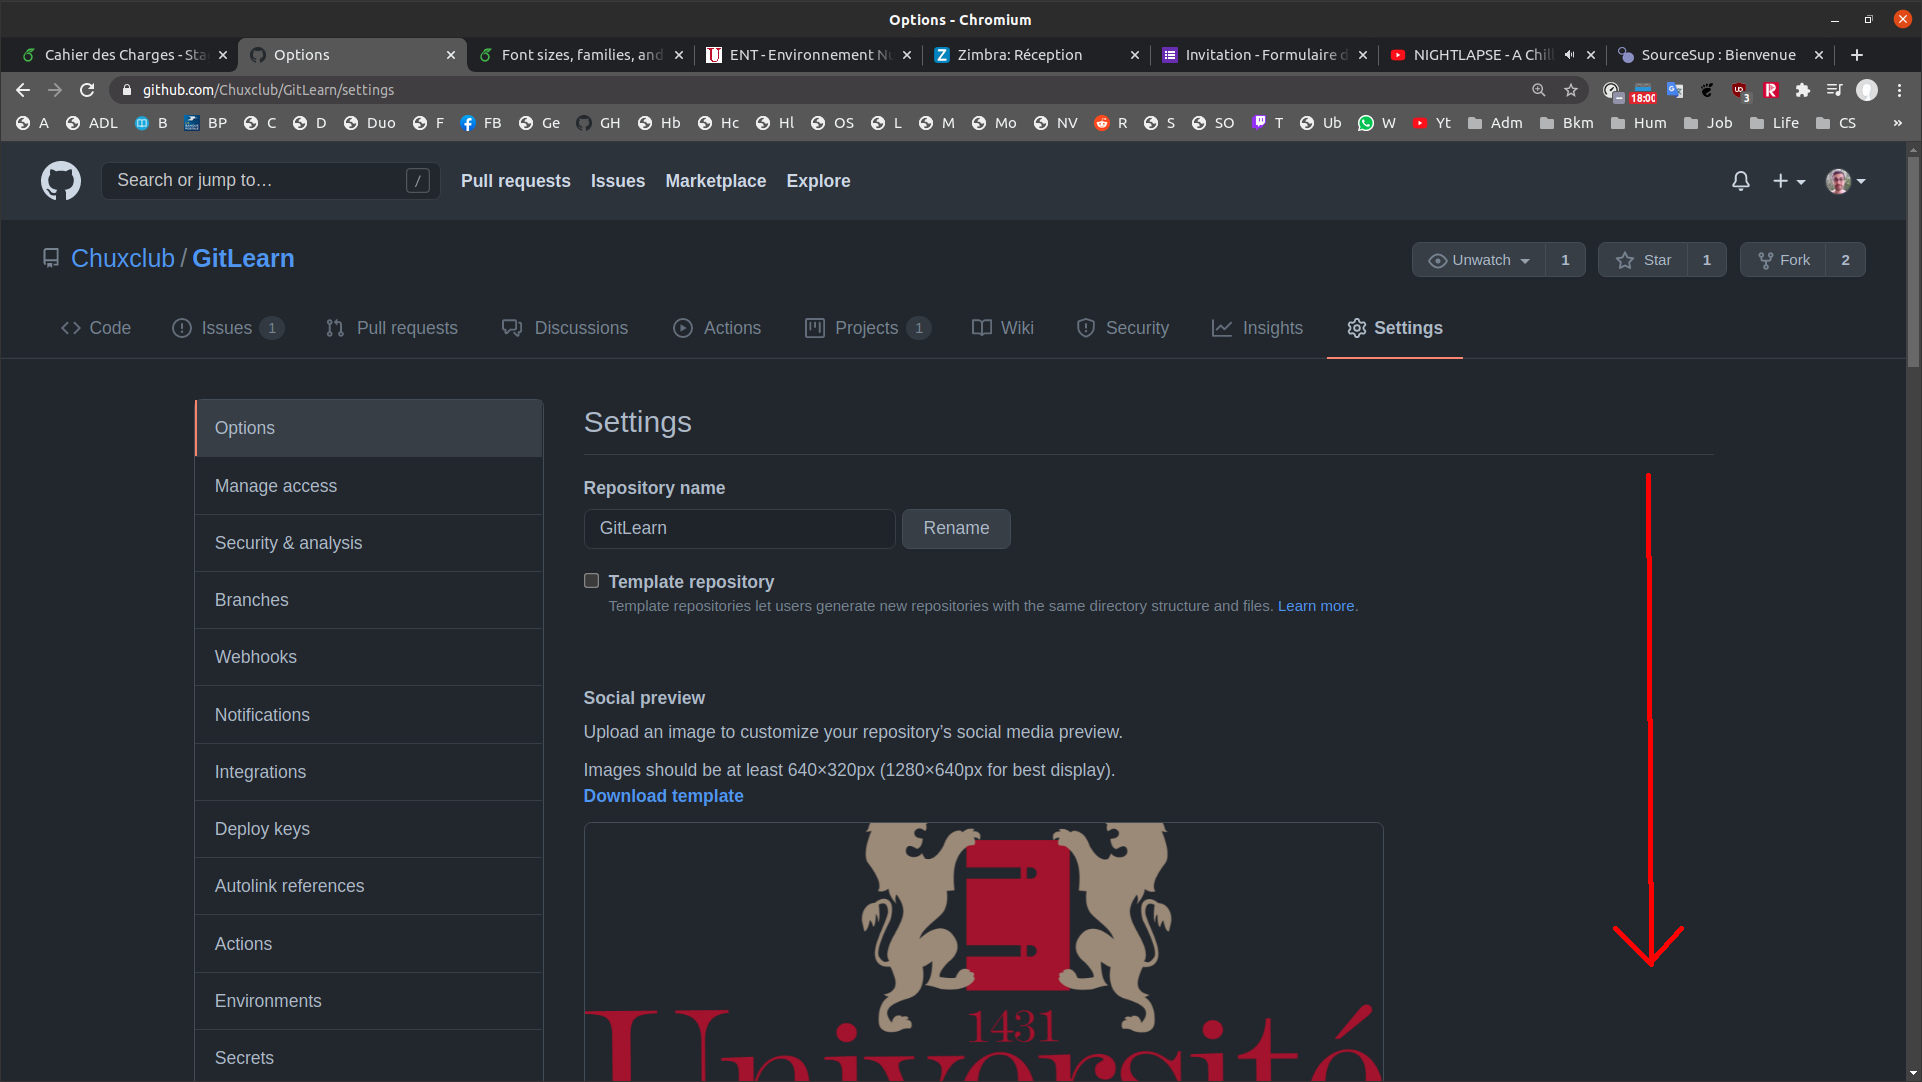
\includegraphics[scale=0.15]{github_options_E.png}
\end{center}
\end{frame}

\begin{frame}{Régler la visibilité après la création du dépôt}
\begin{center}
	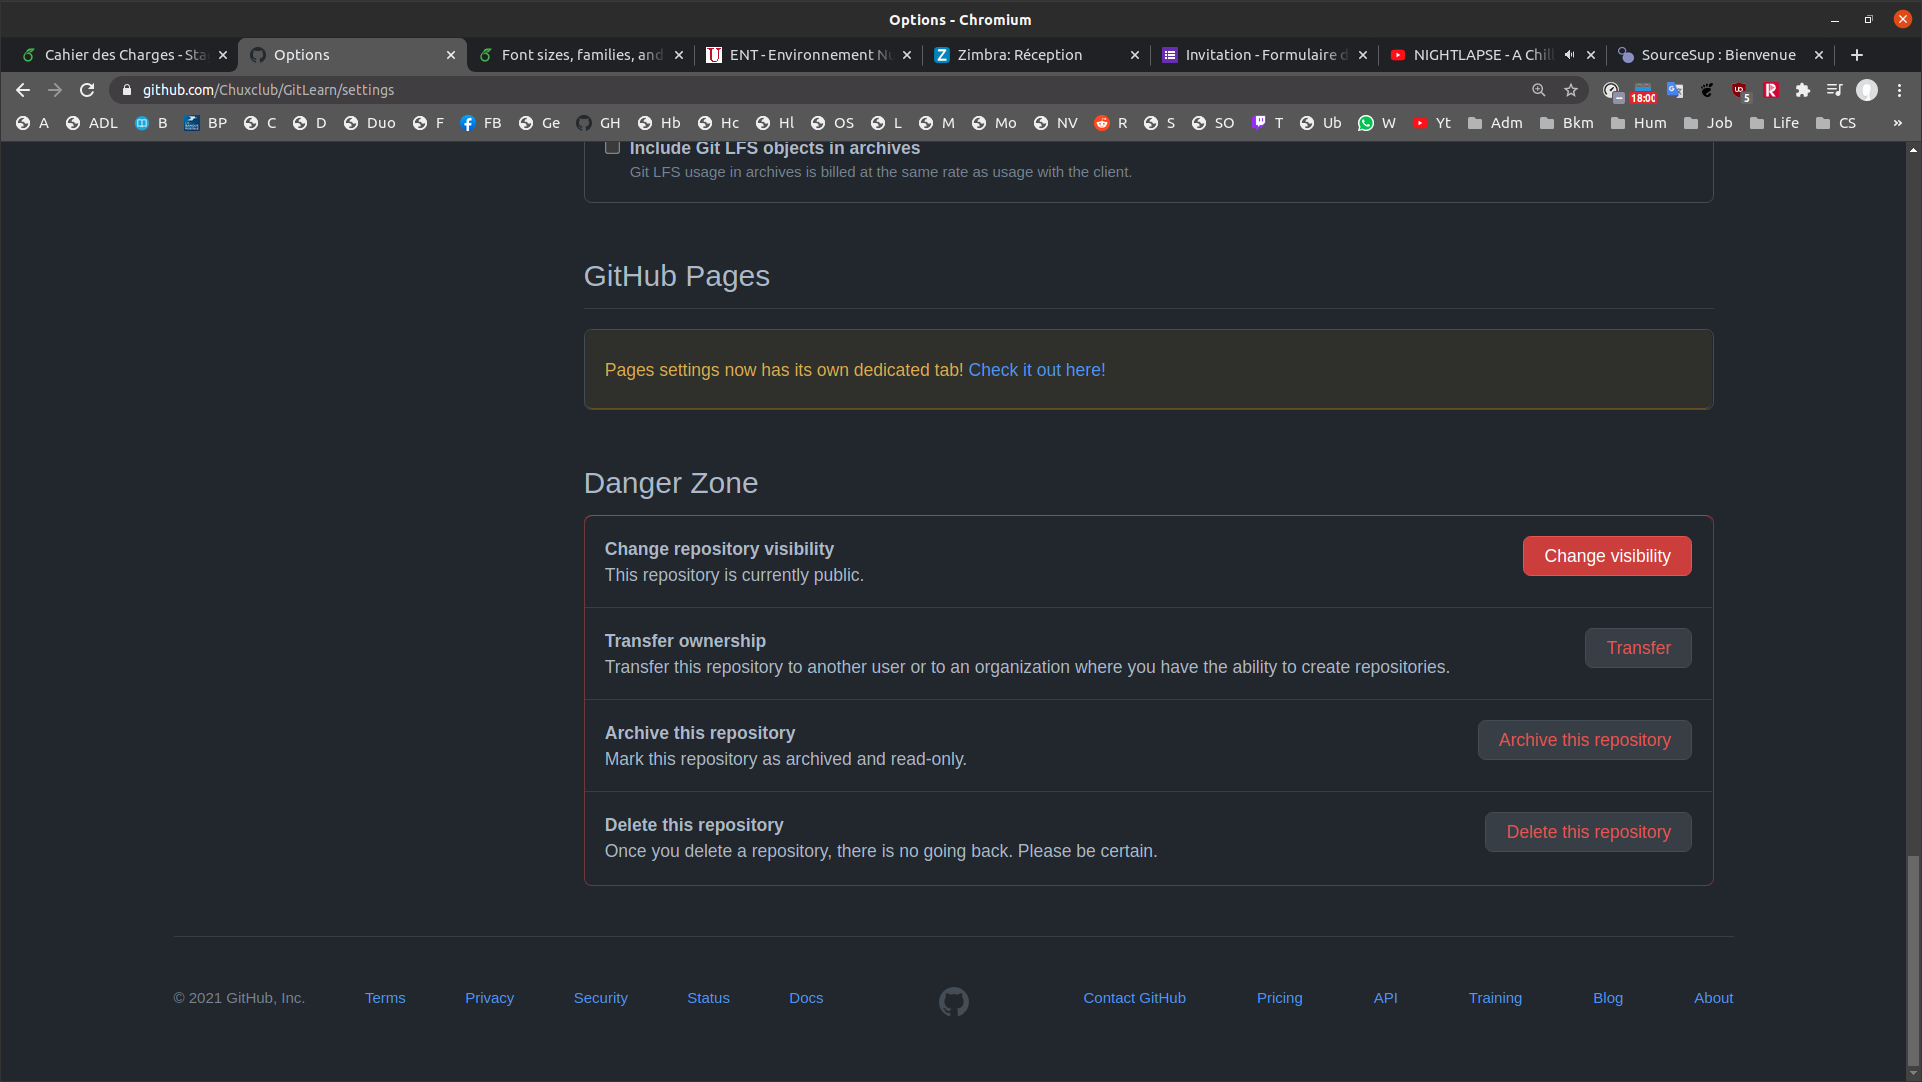
\includegraphics[scale=0.15]{github_visibility.png}
\end{center}
\end{frame}

% Subsection:
\subsection{Collaborer}
\begin{frame}{Inviter un collaborateur}
Il y a trois scénarios possibles, qui dépendent de la configuration du ou des dépôts distants.
\medskip

\underline{Premier scénario:}\\
\smallskip
Vous êtes indiqué comme \textbf{collaborateur} sur la branche distante. En tant que collaborateur vous pouvez "pusher" les changements que vous voulez sans restriction ! Sauf si le projet fait partie d'une organisation...\\
\medskip
\textbf{ATTENTION pour les chefs de projet:} Cela nécessite d'avoir une très grande confiance en ses collaborateurs. En cas de doute une des solutions est alors d'avoir une branche distante de développement
\end{frame}

\begin{frame}{Inviter un collaborateur}

\begin{center}
\begin{figure}[h!]
    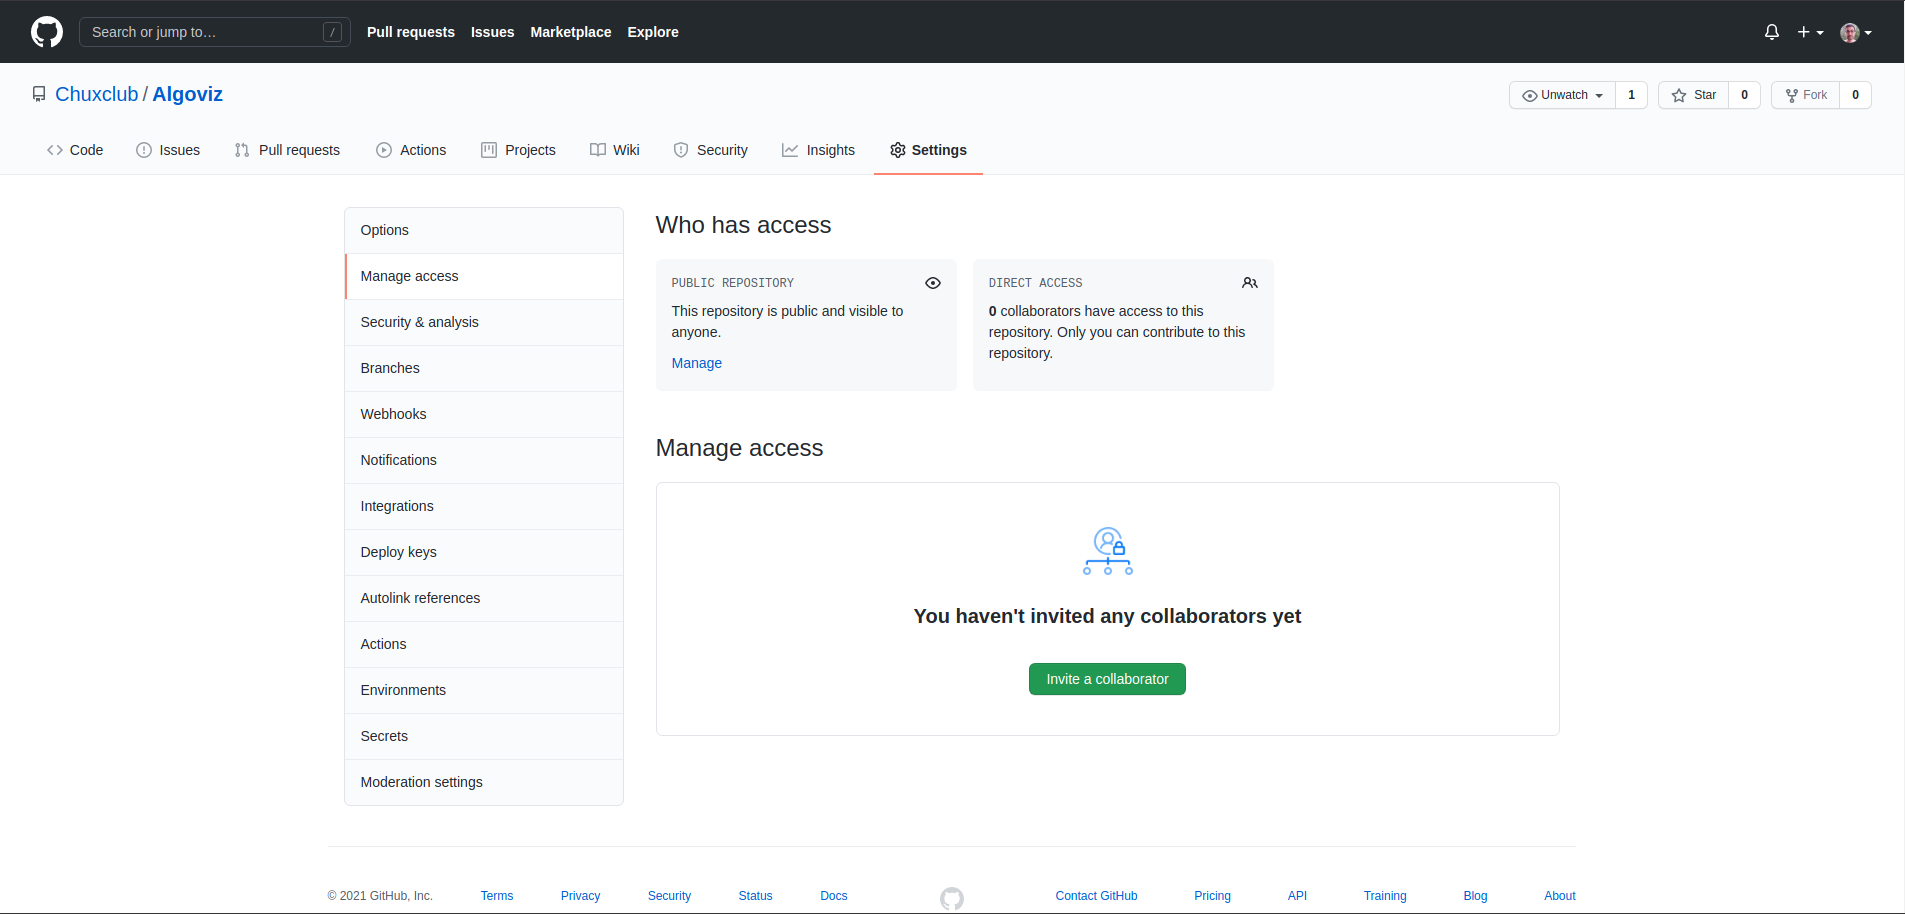
\includegraphics[scale=0.15]{images/droits_push/collaborator.png}
    \caption{Définir des collaborateurs sous GitHub}
\end{figure}
\end{center}

\end{frame}

\begin{frame}{Fork et Pull request}

\underline{Second scénario:}\\
\smallskip

\begin{enumerate}
    \item Vous avez "\textbf{forké}" (càd copié) sous Github le projet d'une personne.
    \item Vous avez ensuite cloné ce fork.
    \item Vous avez travaillé sur ce clone et "pushé" vos projets sur votre fork distant.
    \item Vous pouvez ensuite faire un pull request directement sur l'interface GitHub.
\end{enumerate}

\normalsize
\end{frame}

\begin{frame}{Fork et Pull request}
\begin{figure}[h!]
    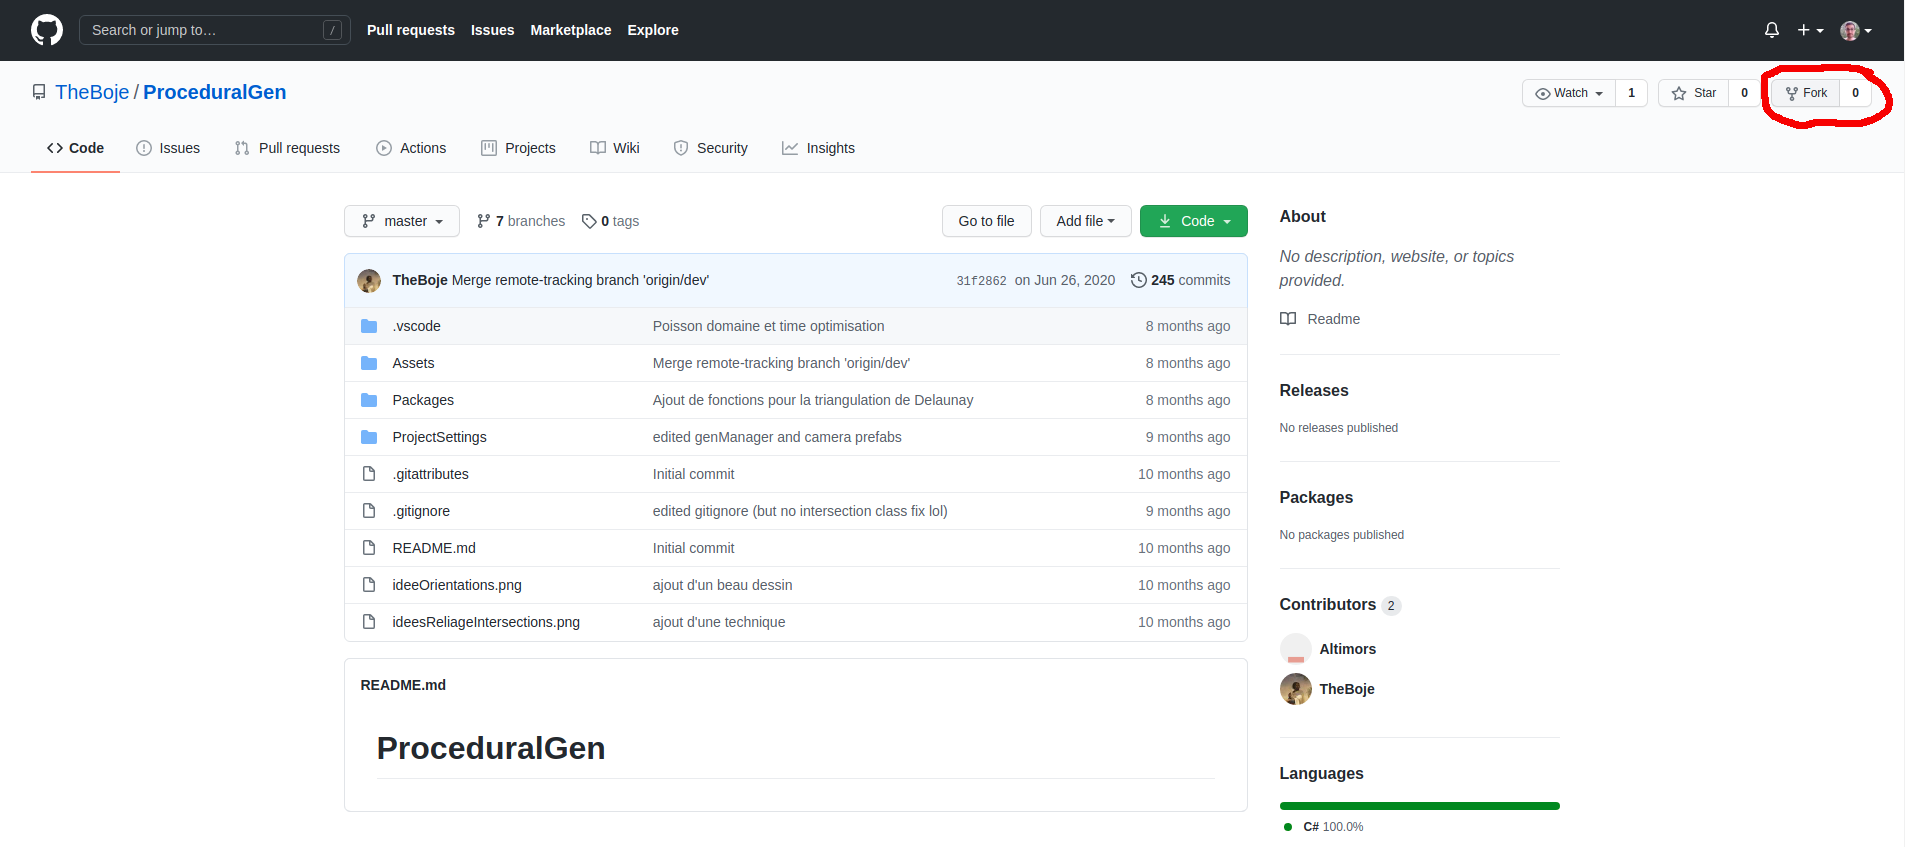
\includegraphics[scale=0.15]{images/droits_push/fork.png}
    \caption{Forker sous GitHub}
\end{figure}
\end{frame}

\begin{frame}{Fork et Pull request}
\begin{figure}[h!]
    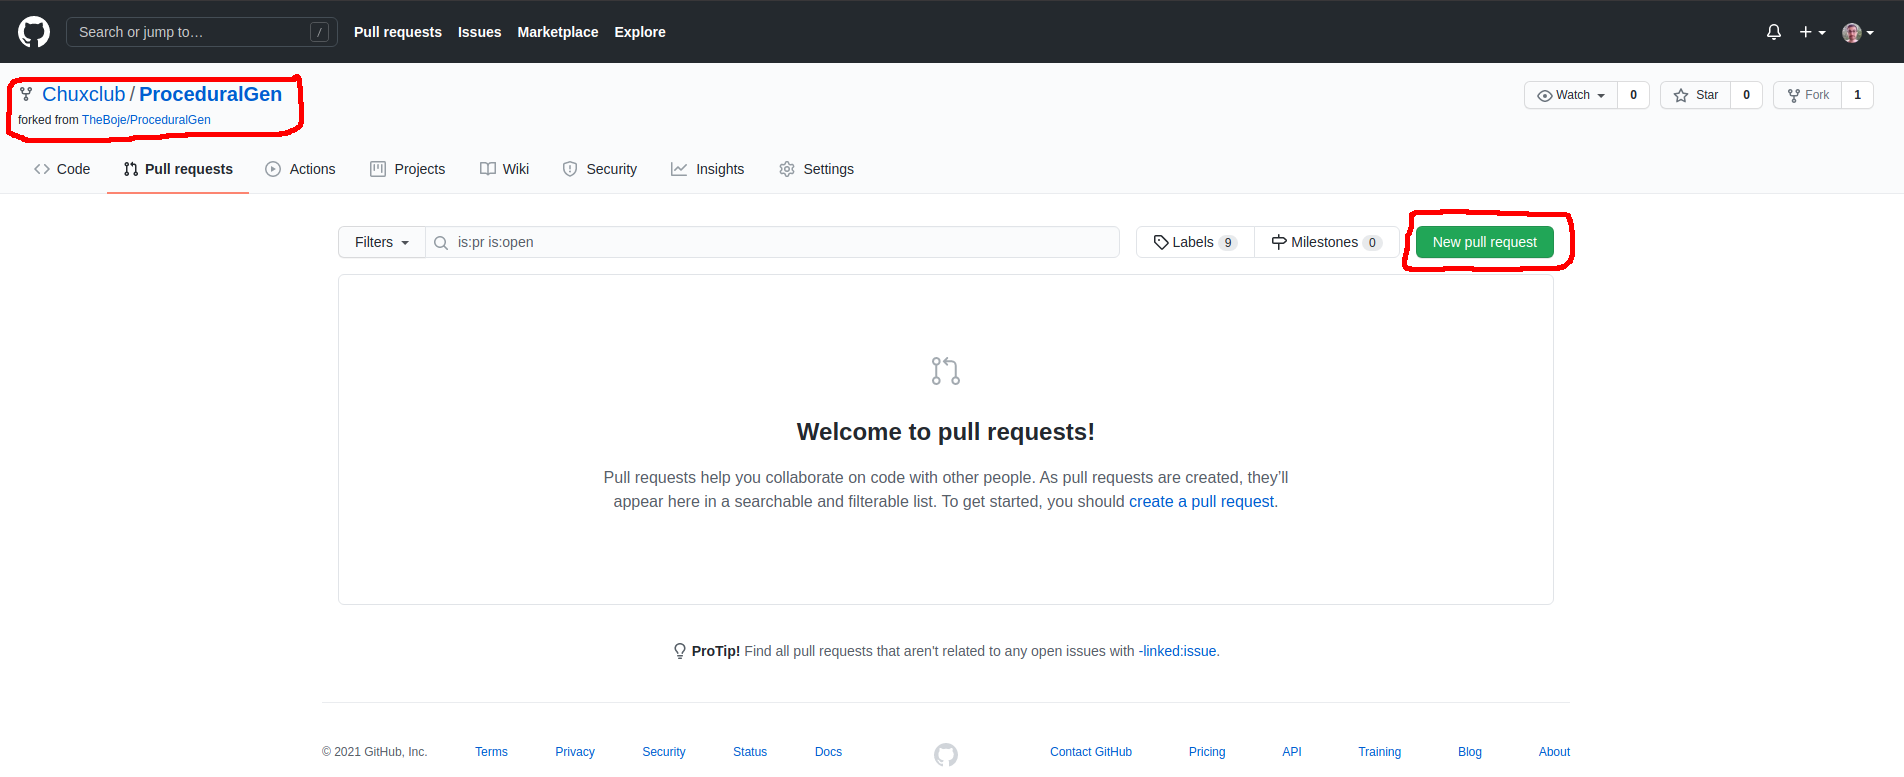
\includegraphics[scale=0.15]{images/droits_push/pull_request.png}
    \caption{Faire un pull request sous GitHub}
\end{figure}
\end{frame}


\begin{frame}{Fork tardif}

\underline{Dernier scénario:}\\
\smallskip
Vous avez \textbf{cloné} le projet d'une personne. Vous avez ensuite travaillé dessus et vous vous rendez compte que vous souhaiteriez faire part de vos modifications à l'auteur...\\
\medskip

\begin{enumerate}
    \item Comme précédemment vous forkez
    \item Vous ajoutez une branche distante à votre clone: \textit{git remote add <nom> <urlDeVotreDepot>} ou, plus brutal: \textit{git remote rm origin} suivi de \textit{git remote add origin <urlDeVotreDepot>}
    \item Vous pushez vos changements sur ce fork
    \item Vous faites un pull request comme précédemment
\end{enumerate}
\end{frame}




%% --------------------- %%
%%        SECTION        %%
%% --------------------- %%
\AtBeginSection[]
{
  \begin{frame}
    \frametitle{Table of Contents}
    \tableofcontents[sectionstyle=show/hide,subsectionstyle=show/show/hide]
  \end{frame}
}


\section{Communiquer autour du projet avec GitHub}

% Subsection:
\subsection{Communiquer}
\begin{frame}{Les notifications}
Les notifications permettent à celles et ceux qui y sont inscrits de recevoir des mails dès qu'une mise à jour est faite sur le projet:
\begin{center}
	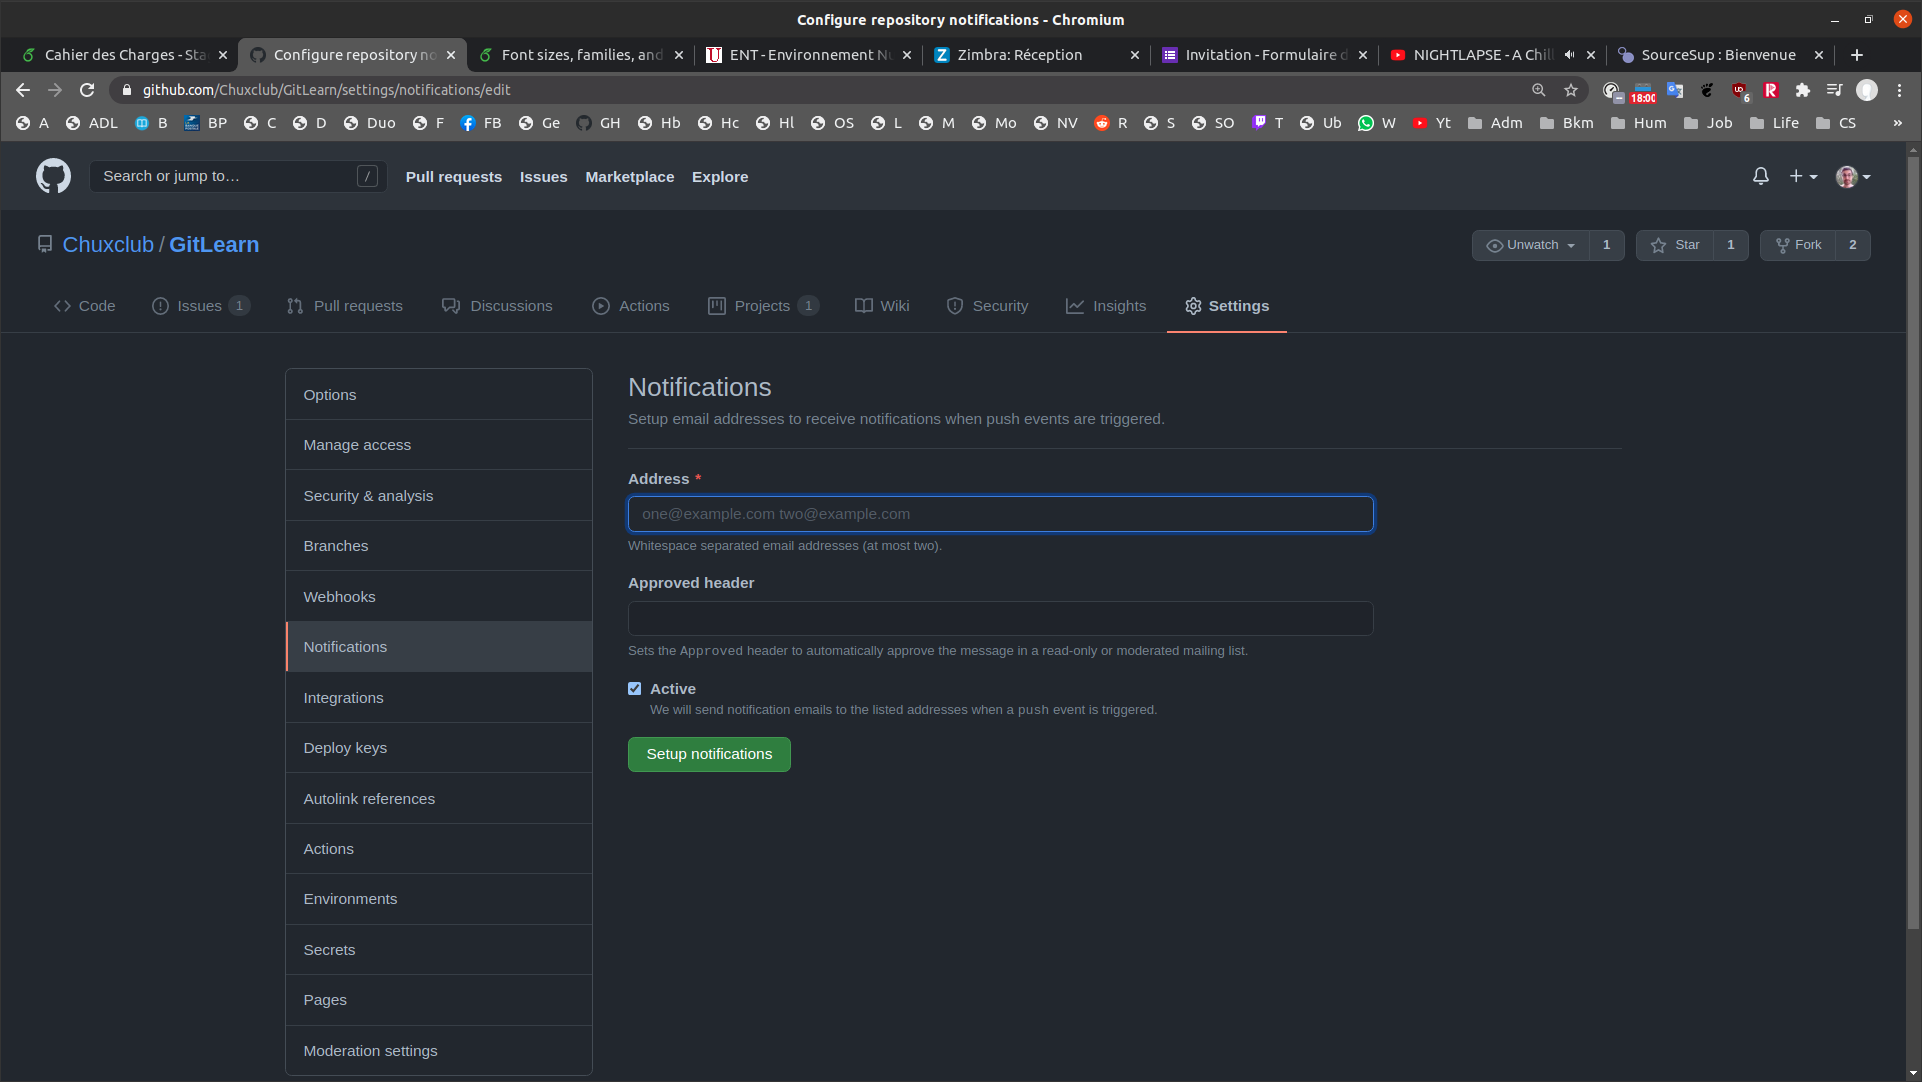
\includegraphics[scale=0.15]{github_notifications.png}
\end{center}
\end{frame}

\begin{frame}{Les discussions}
Les discussions sont des sortes de listes de diffusion de mails avec des sujets fixes:
\begin{center}
	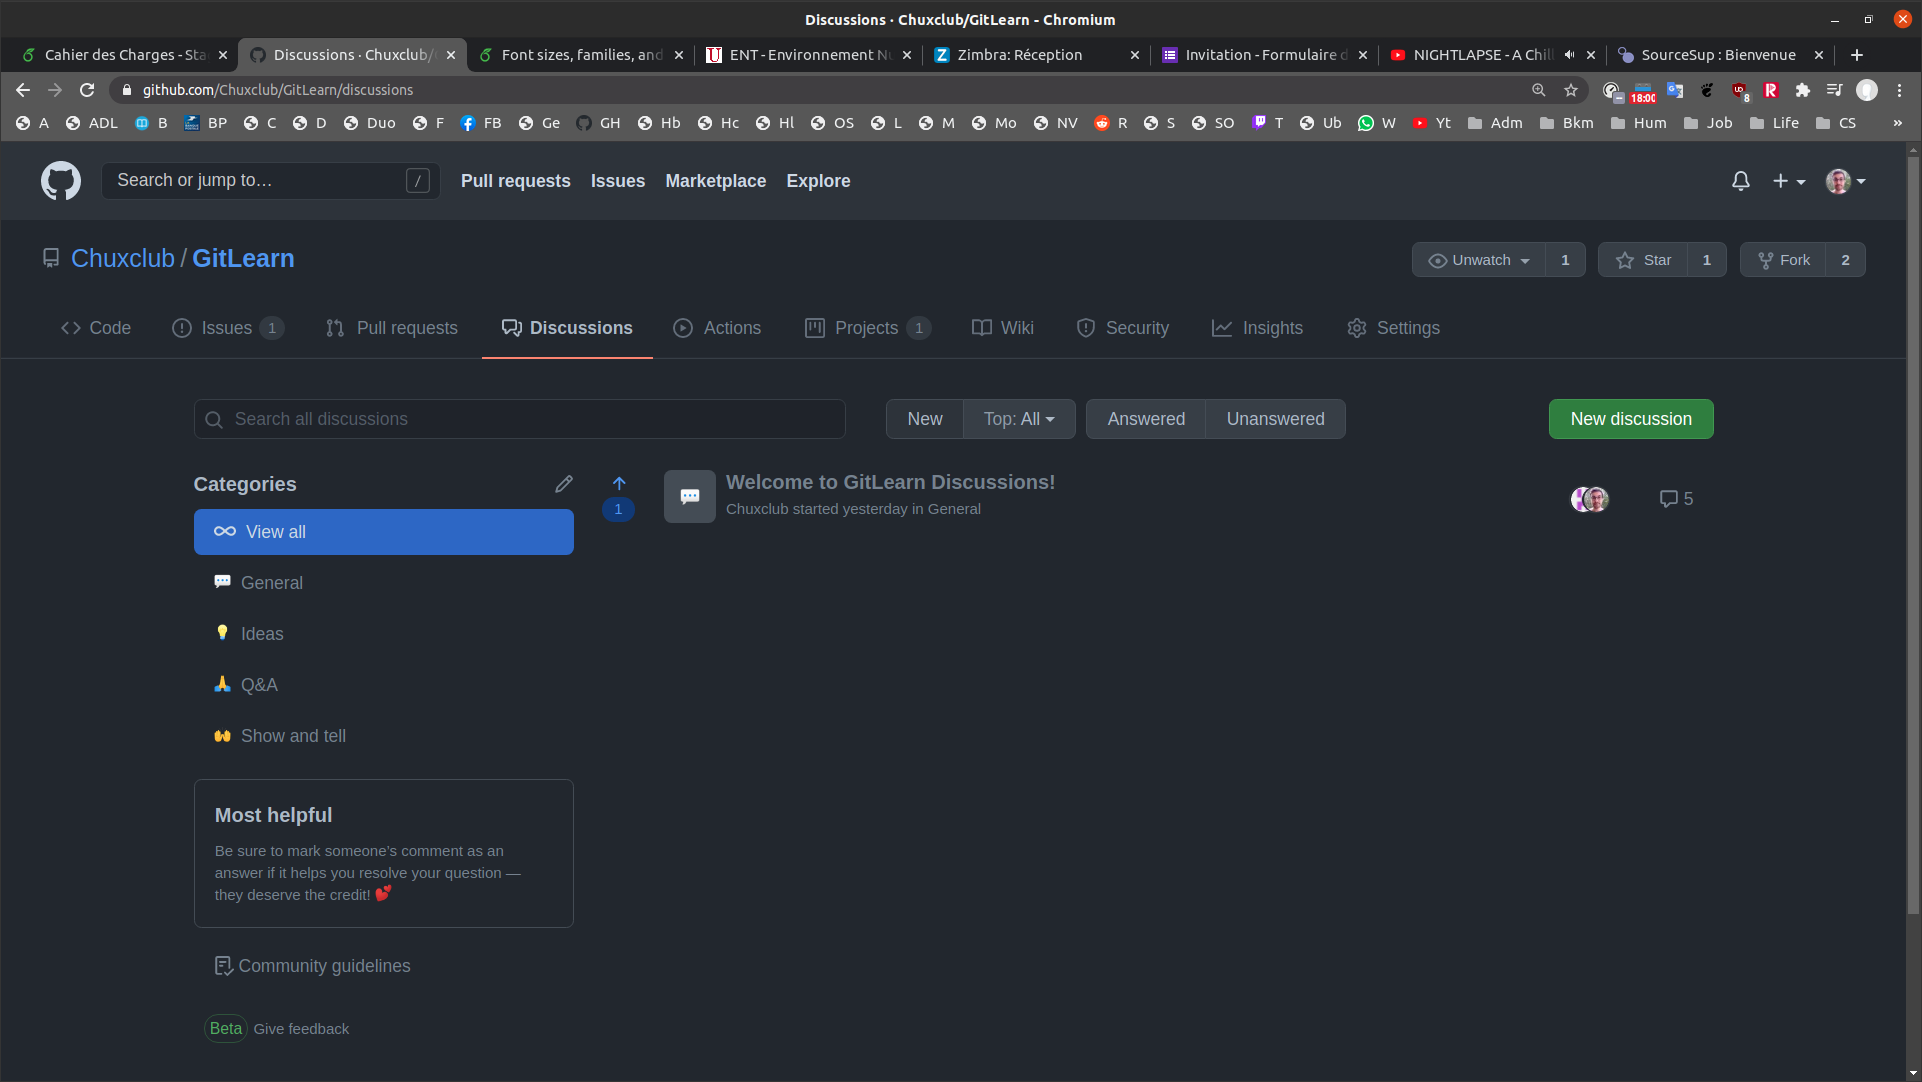
\includegraphics[scale=0.15]{github_discussions1.png}
\end{center}
\end{frame}

\begin{frame}{Les discussions}
Il est possible de désabonner d'une discussion pour cesser de recevoir des mails ou au contraire d'épingler celle-ci pour qu'elle reste visible à tout moment:
\begin{center}
	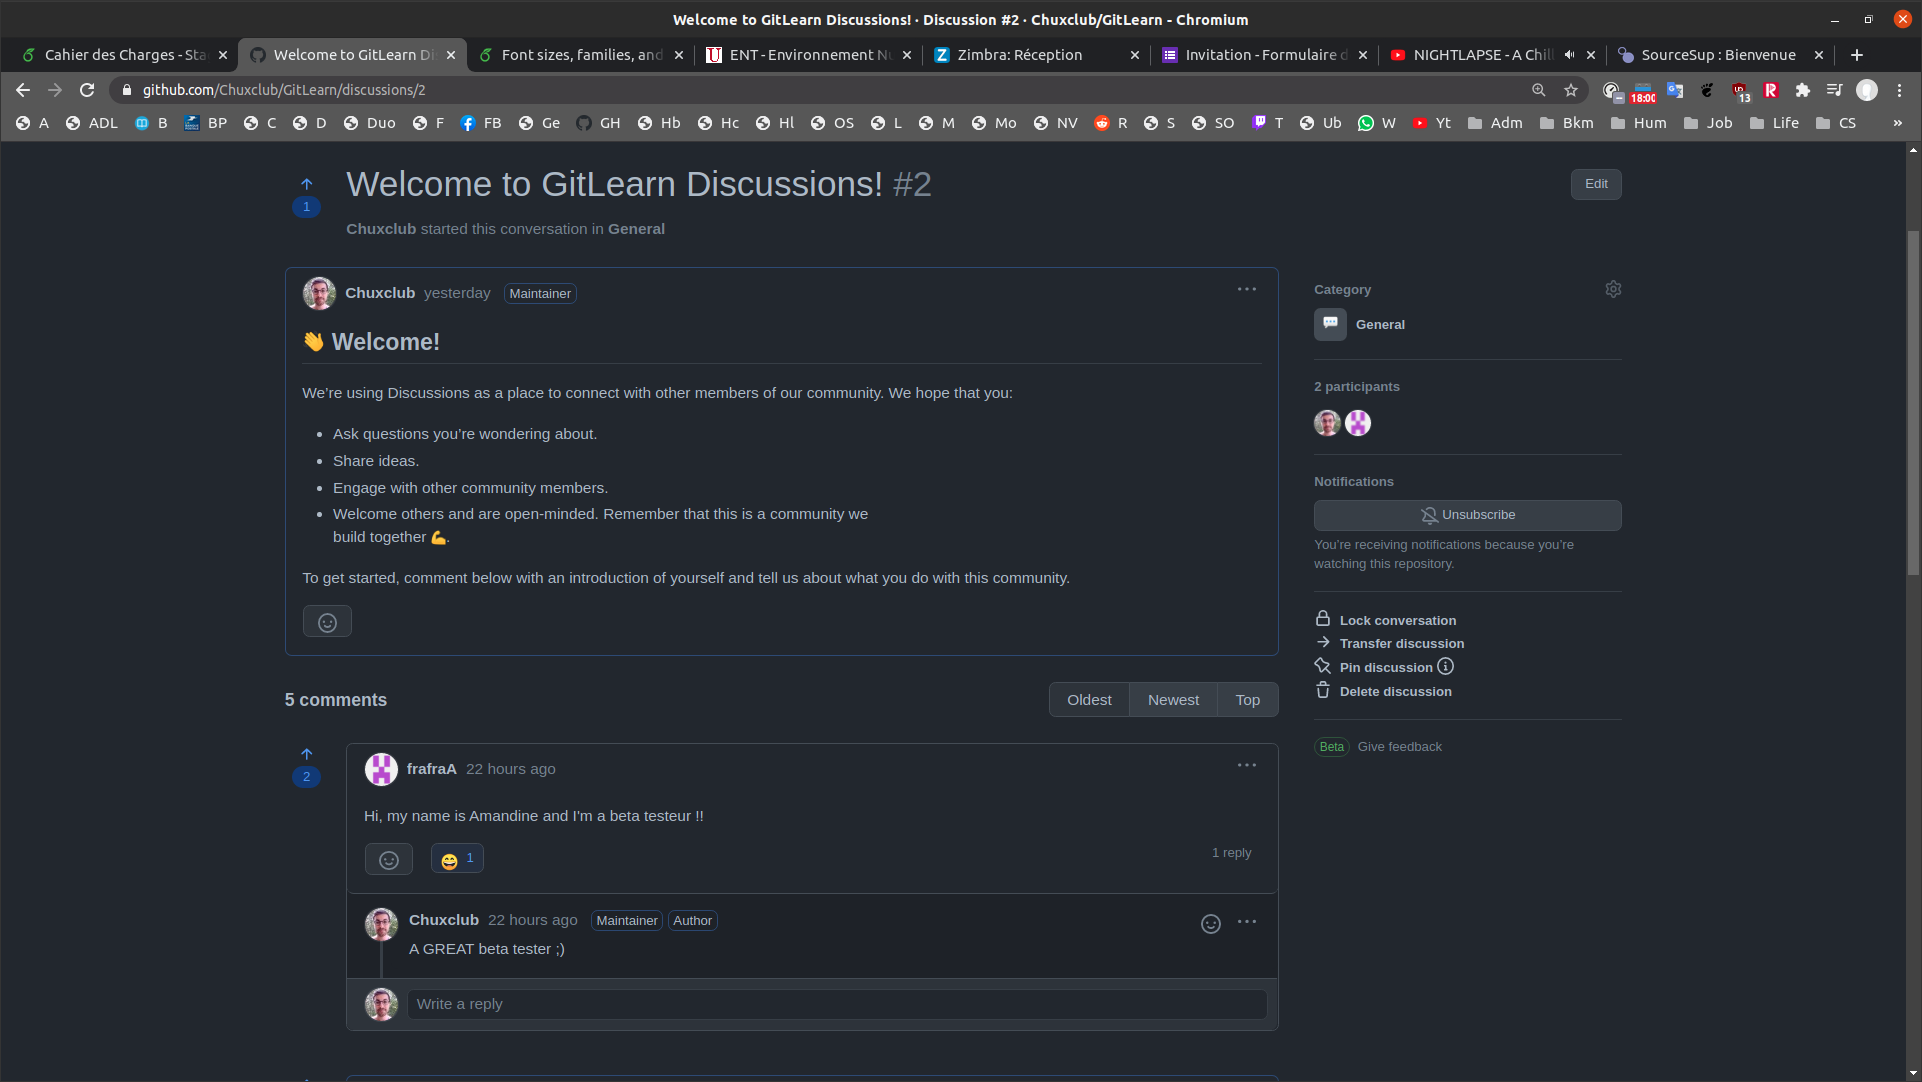
\includegraphics[scale=0.15]{github_discussions2.png}
\end{center}
\end{frame}

\begin{frame}{Les discussions}
Il est possible d'y répondre directement depuis sa boîte mail:
\begin{center}
	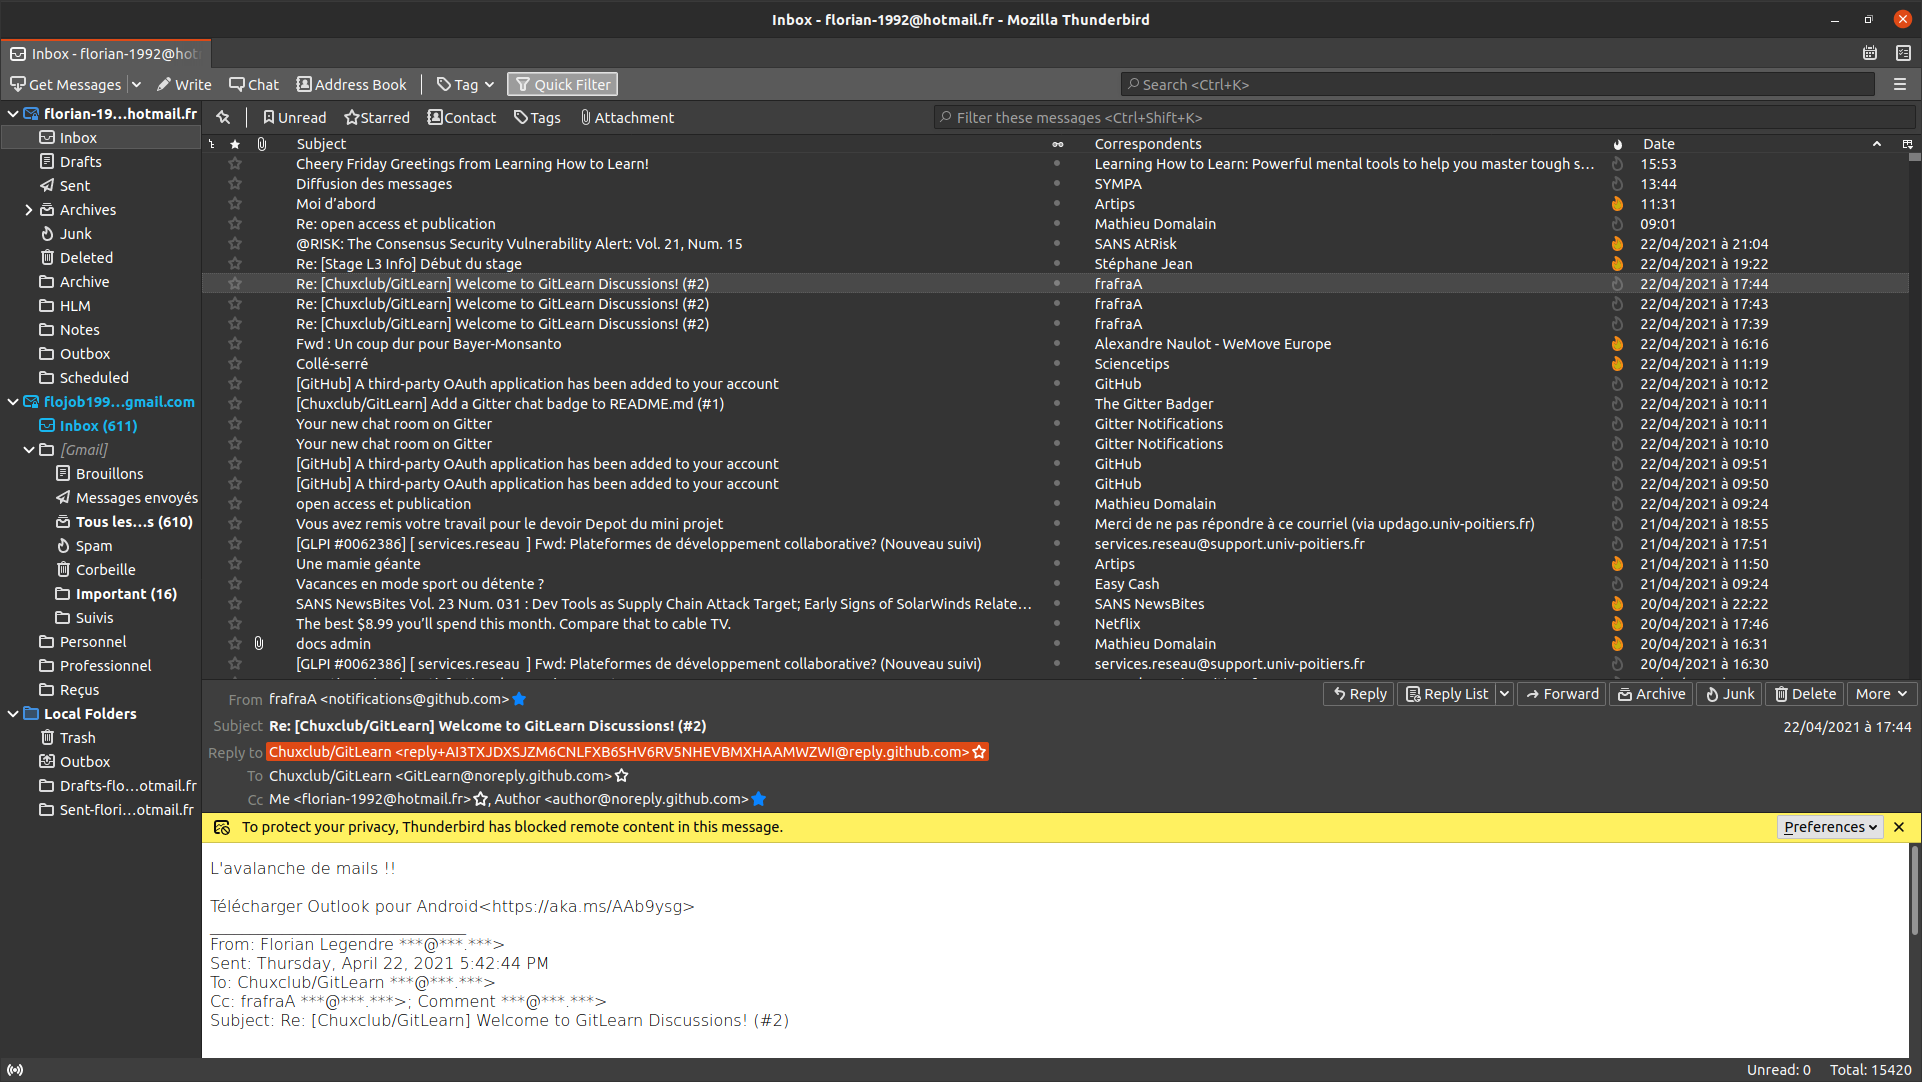
\includegraphics[scale=0.15]{github_discussions3.png}
\end{center}
\end{frame}

\begin{frame}{Les tickets (ou issues)}
Un ticket est un moyen d'indiquer qu'une feature est souhaitée ou un bug a été détecté ou même tout simplement de poser une question. L'avantage est que ces "billets"/"tickets" peuvent être catégorisés par des labels et triés automatiquement:
\begin{center}
	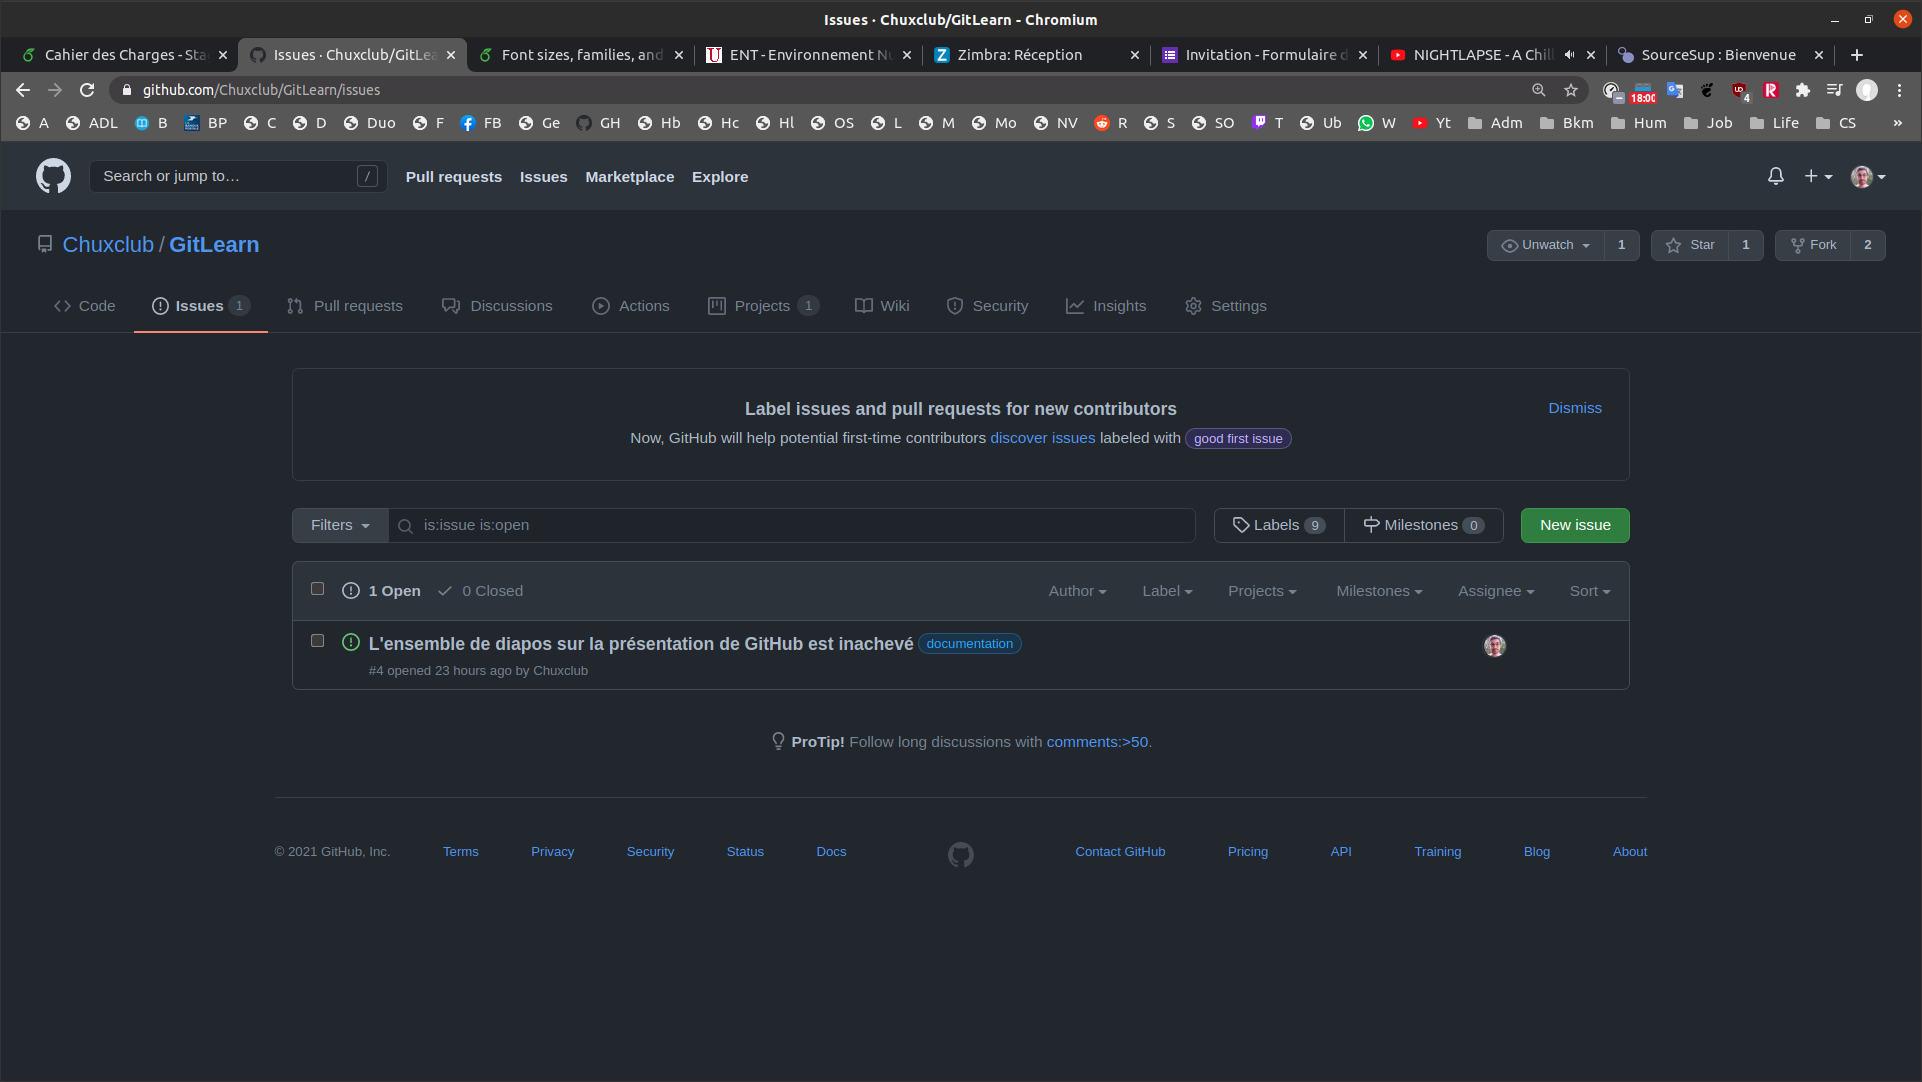
\includegraphics[scale=0.15]{github_issues1.png}
\end{center}
\end{frame}

\begin{frame}{Les tickets (ou issues)}
Il est également possible de créer des templates de tickets (comme pour un bug report) qui permettent de standardiser le contenu de ces-derniers. Il suffit d'aller dans les options de ce-dernier:
\begin{center}
	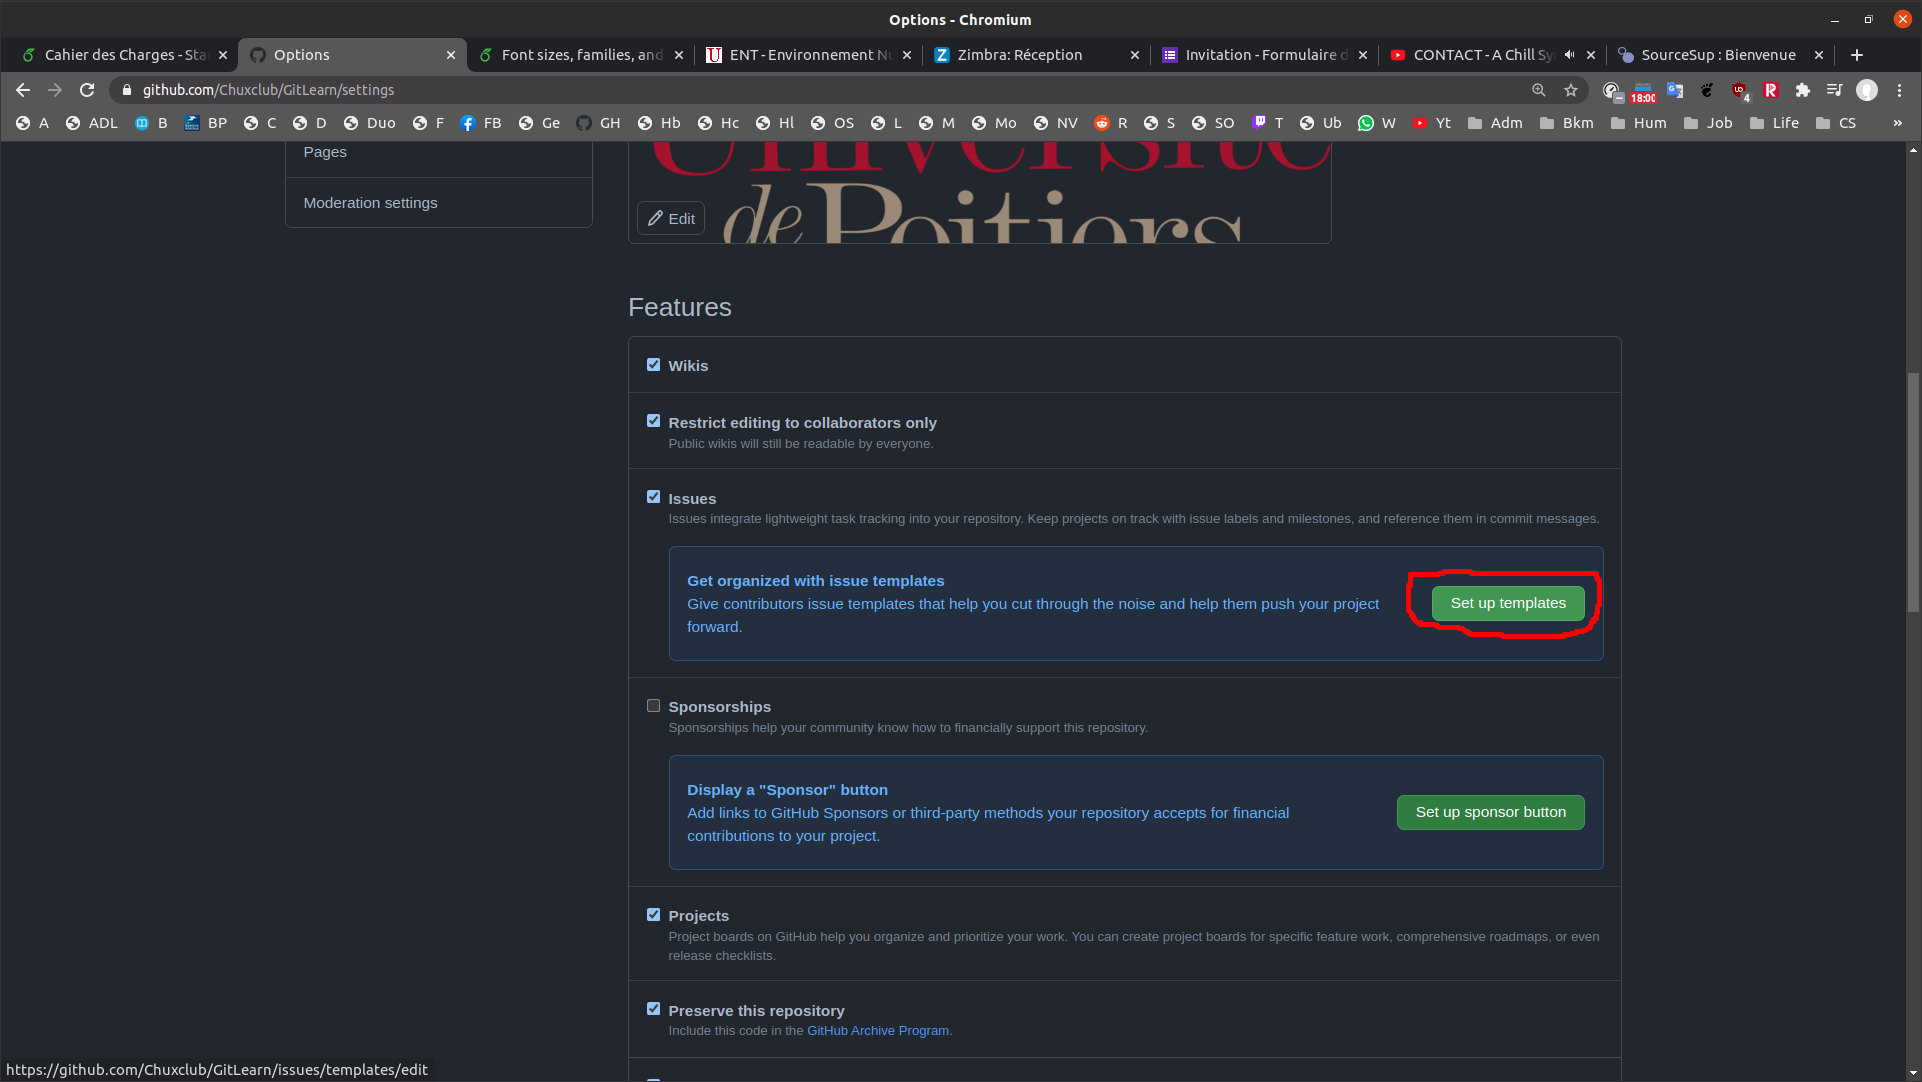
\includegraphics[scale=0.15]{github_issues3_E.png}
\end{center}
\end{frame}


\begin{frame}{Les tickets (ou issues)}
Création d'un billet avec choix du template. Si aucun template ne convient à l'utilisateur il peut choisir de créer un billet sans template:
\begin{center}
	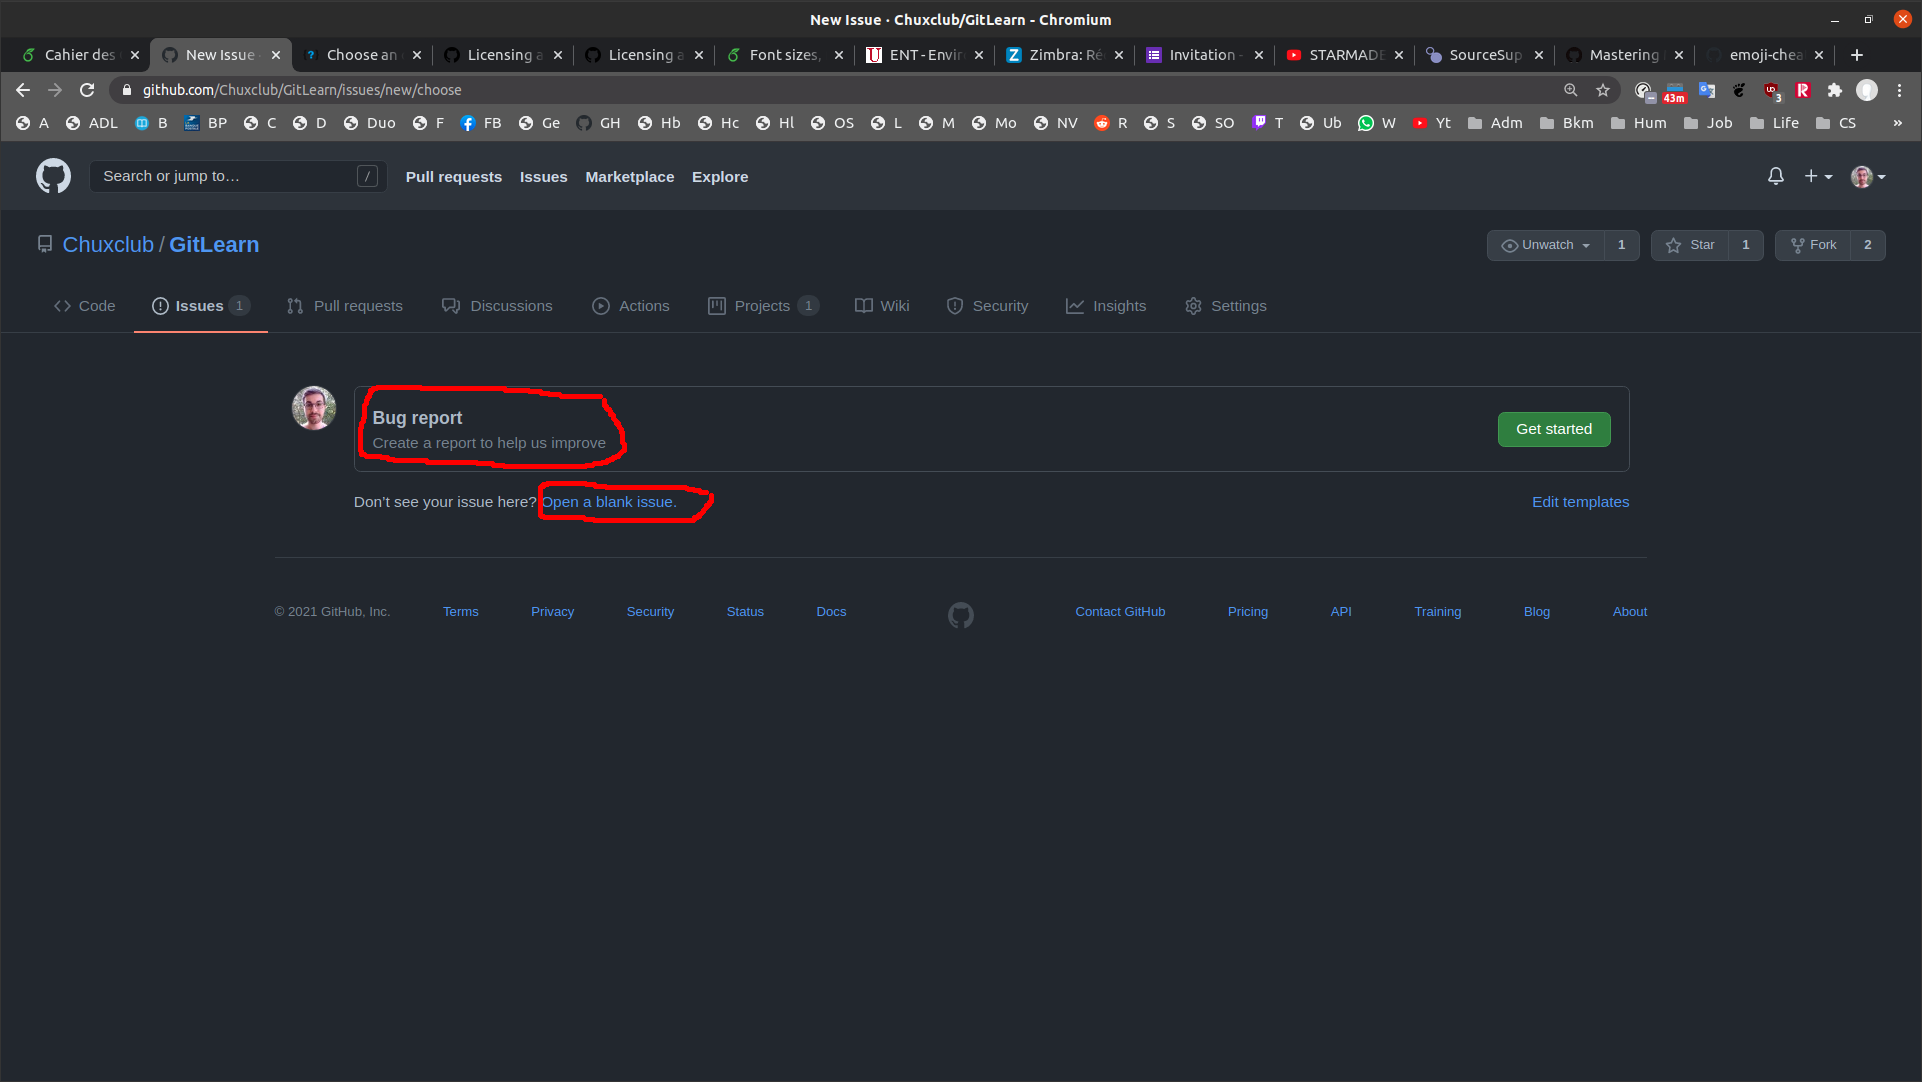
\includegraphics[scale=0.15]{github_issues5_E.png}
\end{center}
\end{frame}

\begin{frame}{Les tickets (ou issues)}
Édition d'un billet avec template:
\begin{center}
	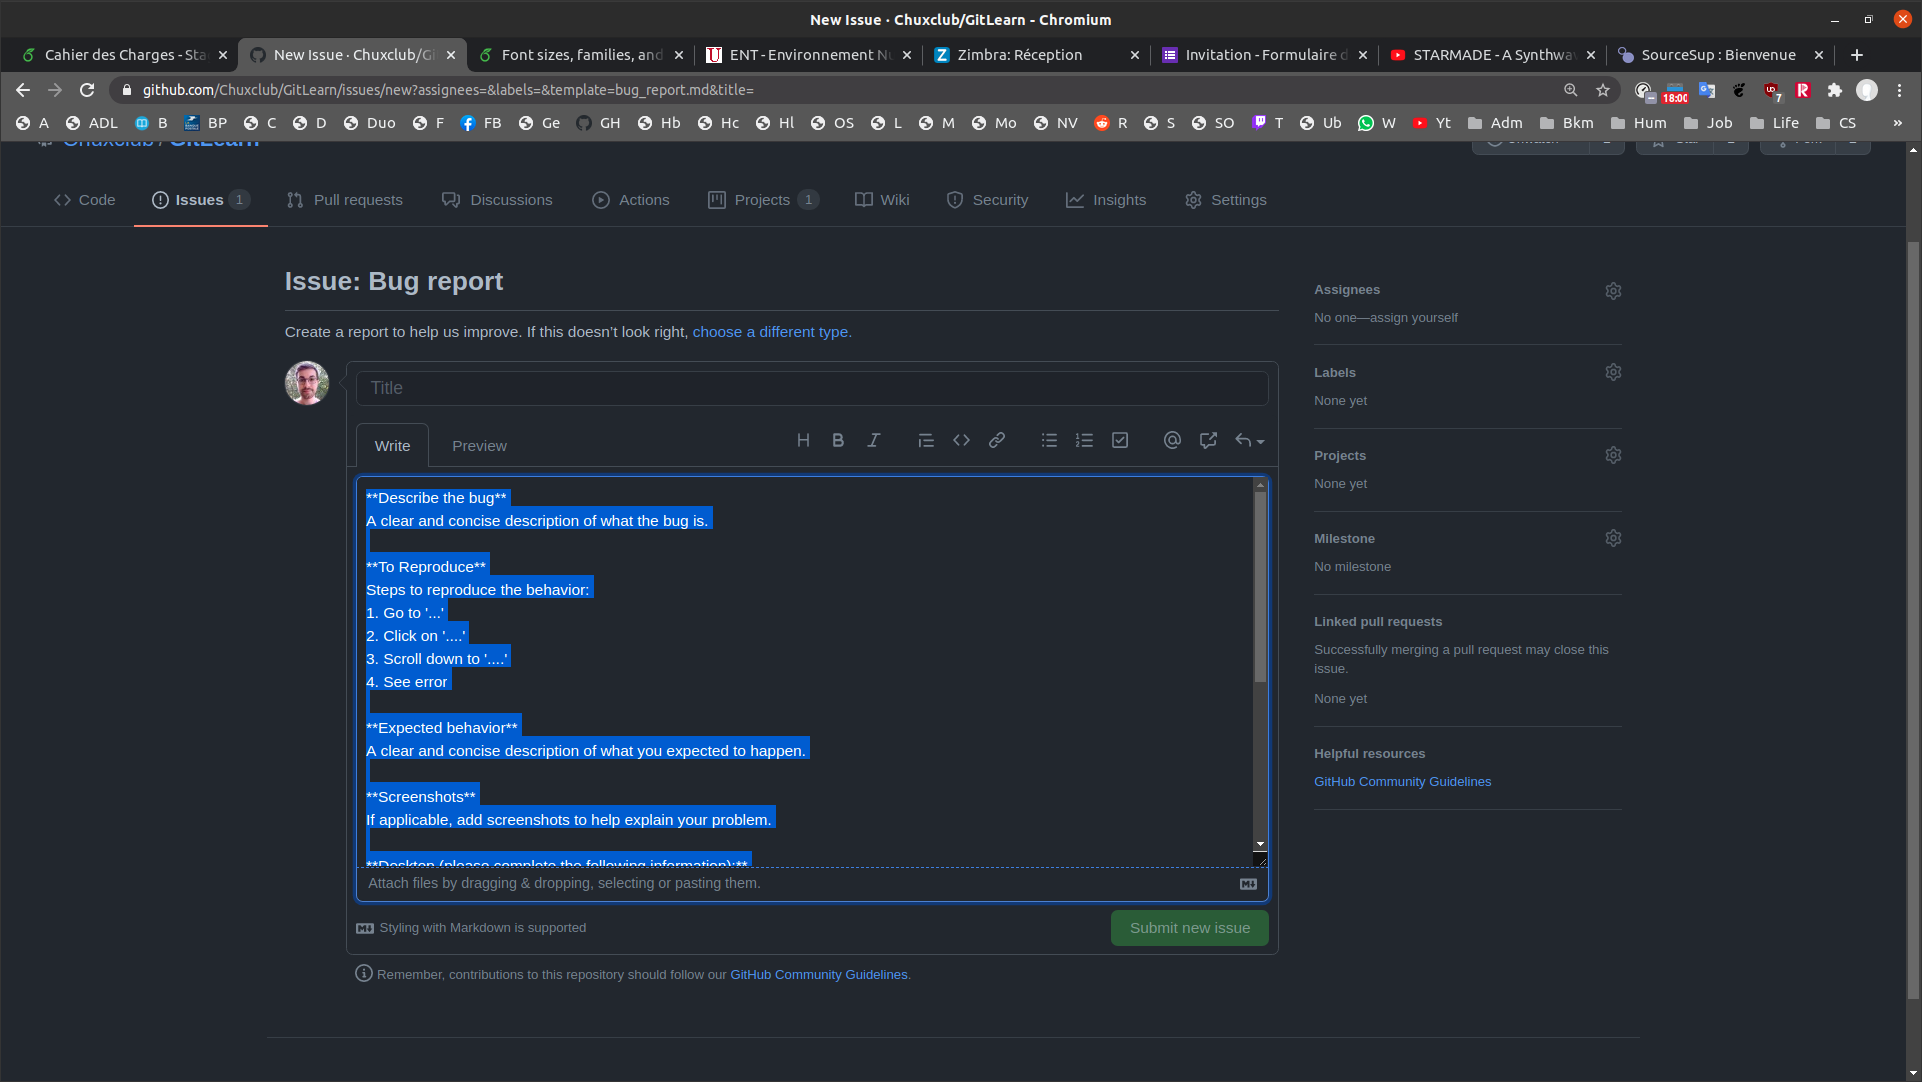
\includegraphics[scale=0.15]{github_issues4.png}
\end{center}
\end{frame}

\begin{frame}{Les tickets (ou issues)}
Édition d'un billet sans template:
\begin{center}
	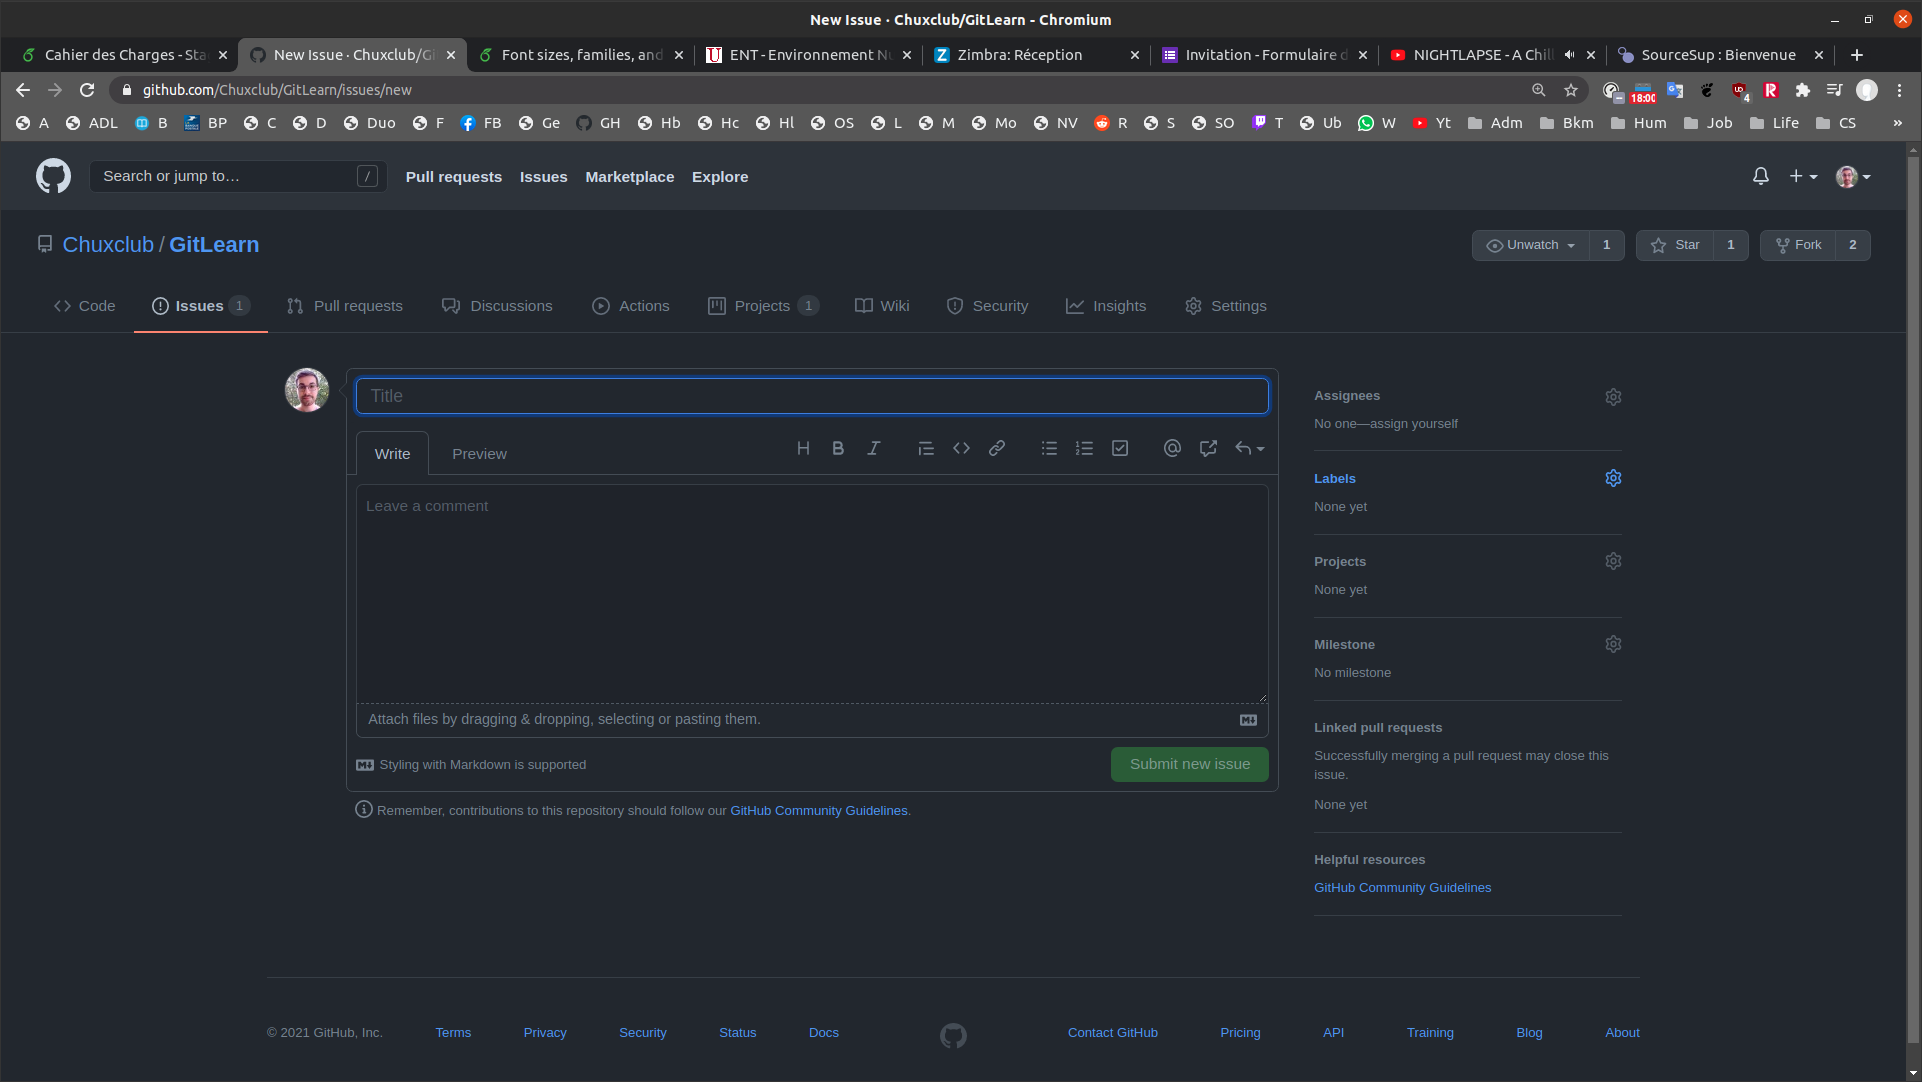
\includegraphics[scale=0.15]{github_issues2.png}
\end{center}
\end{frame}


\begin{frame}{Les projets}
Les projets sont des tableaux de bord de l'avancement du projet. Les tickets peuvent y apparaître automatiquement et triés en colonnes "à faire" / "en cours" / "terminés":
\begin{center}
	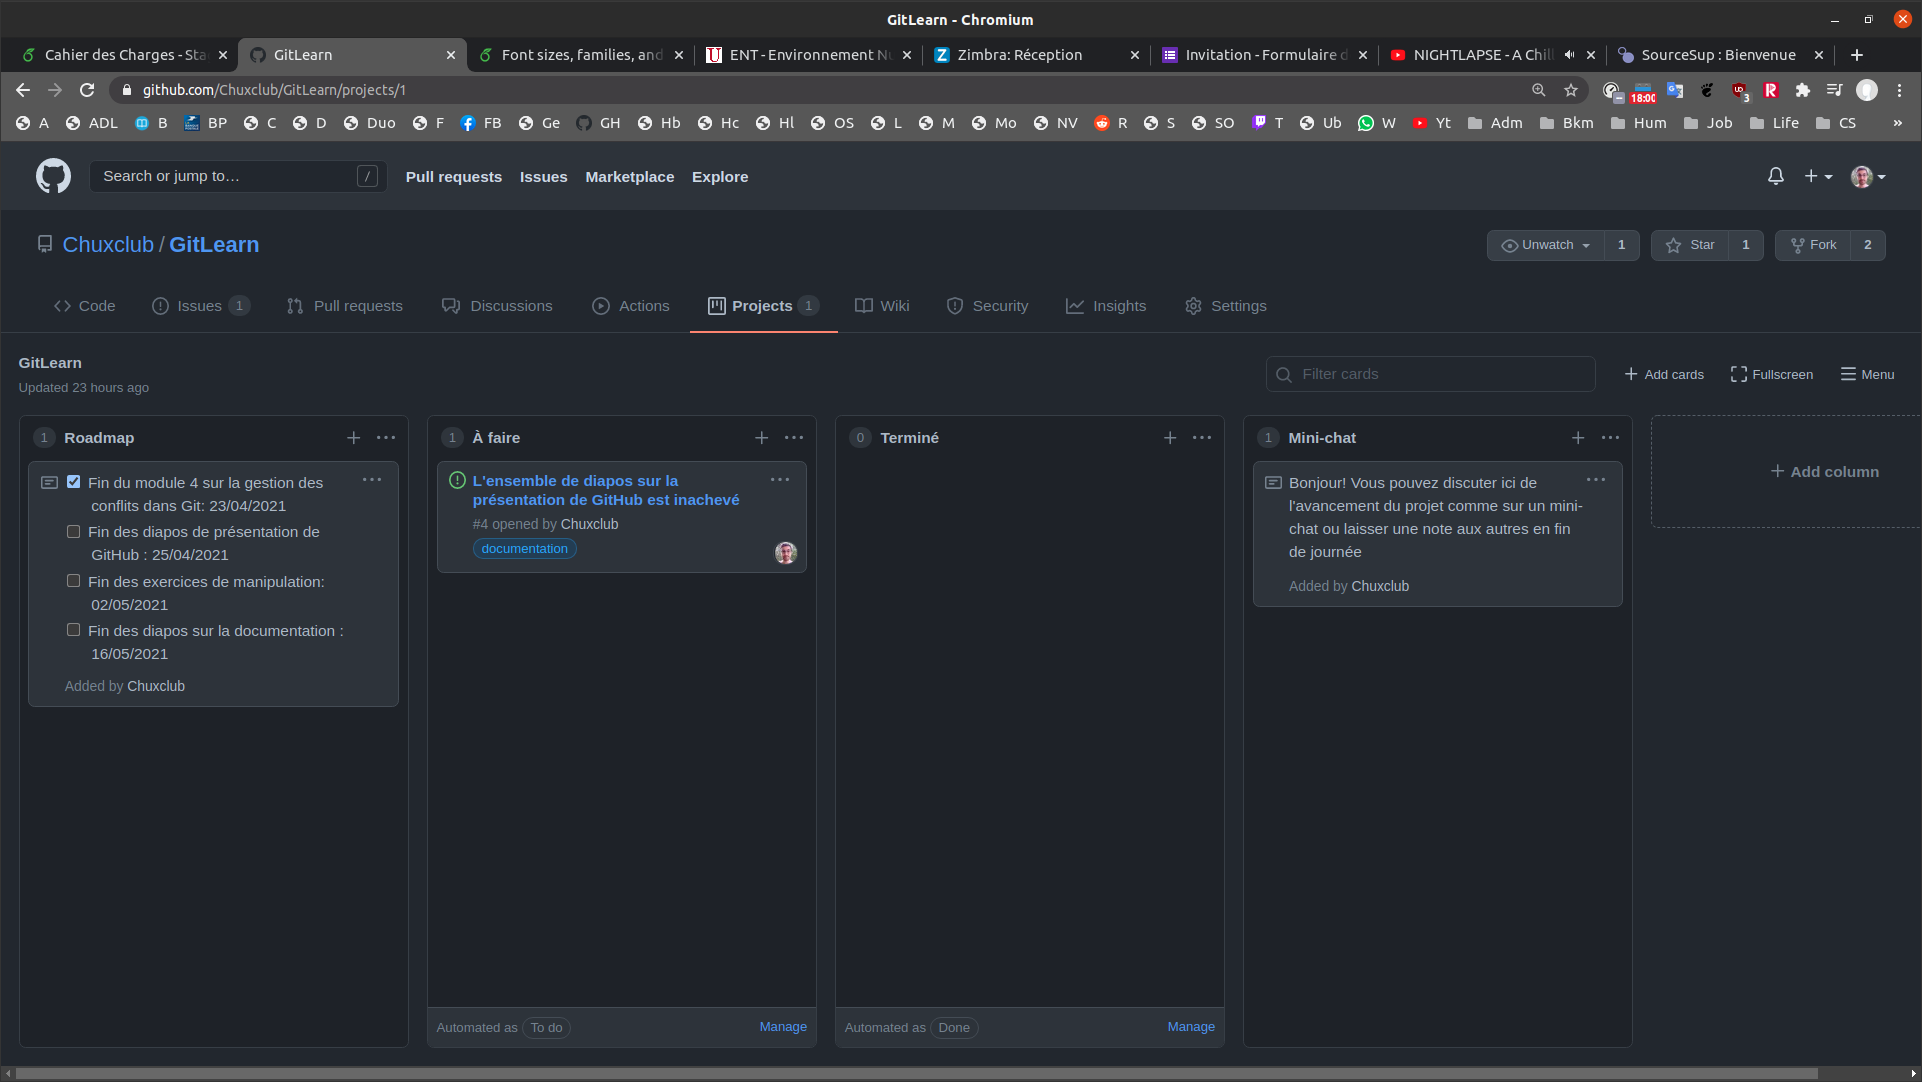
\includegraphics[scale=0.15]{github_projects2.png}
\end{center}
\end{frame}

\begin{frame}
Les projets fonctionnent en utilisant deux briques: les colonnes et dans les colonnes des cartes. Il est possible d'utiliser la syntaxe MarkDown dans ces cartes. Aussi vous pouvez donner le sens et l'usage que vous voulez à vos colonnes:\\
\medskip

\begin{itemize}
	\item Créer une roadmap du projet
	\item Un mini-chat
	\item Une colonne de liens vers des documentations extérieures
	\item Les gestions de tickets
	\item Une colonne "dates importantes" qui donne les deadlines ou la date de la prochaine réunion autour du projet
	\item etc.
\end{itemize}
\end{frame}

\begin{frame}{Les projets}
Il est possible de créer plusieurs projets dans les cas où, par exemple, le projet implique plusieurs gros services différents:
\begin{center}
	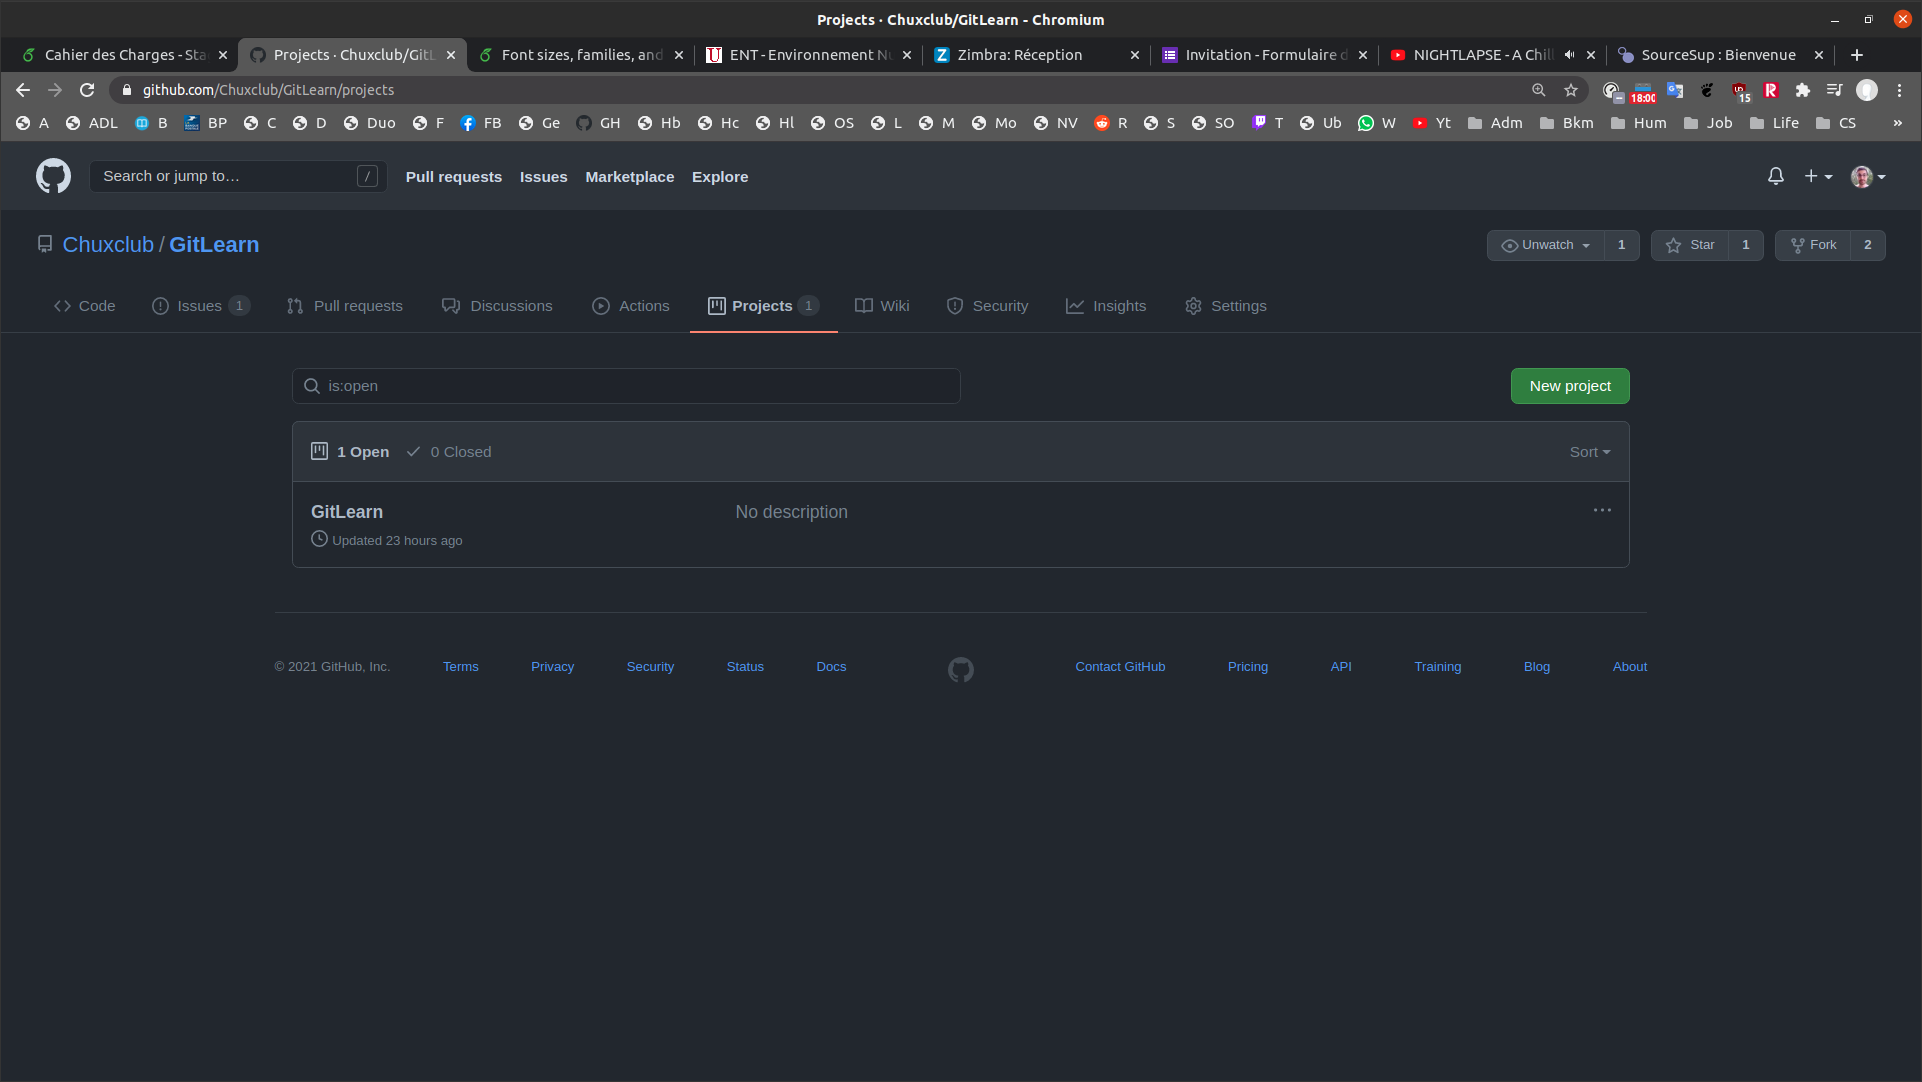
\includegraphics[scale=0.15]{github_projects1.png}
\end{center}
\end{frame}



% Subsection:
\subsection{Les fichiers spéciaux}
\begin{frame}{Le fichier README}
\begin{center}
	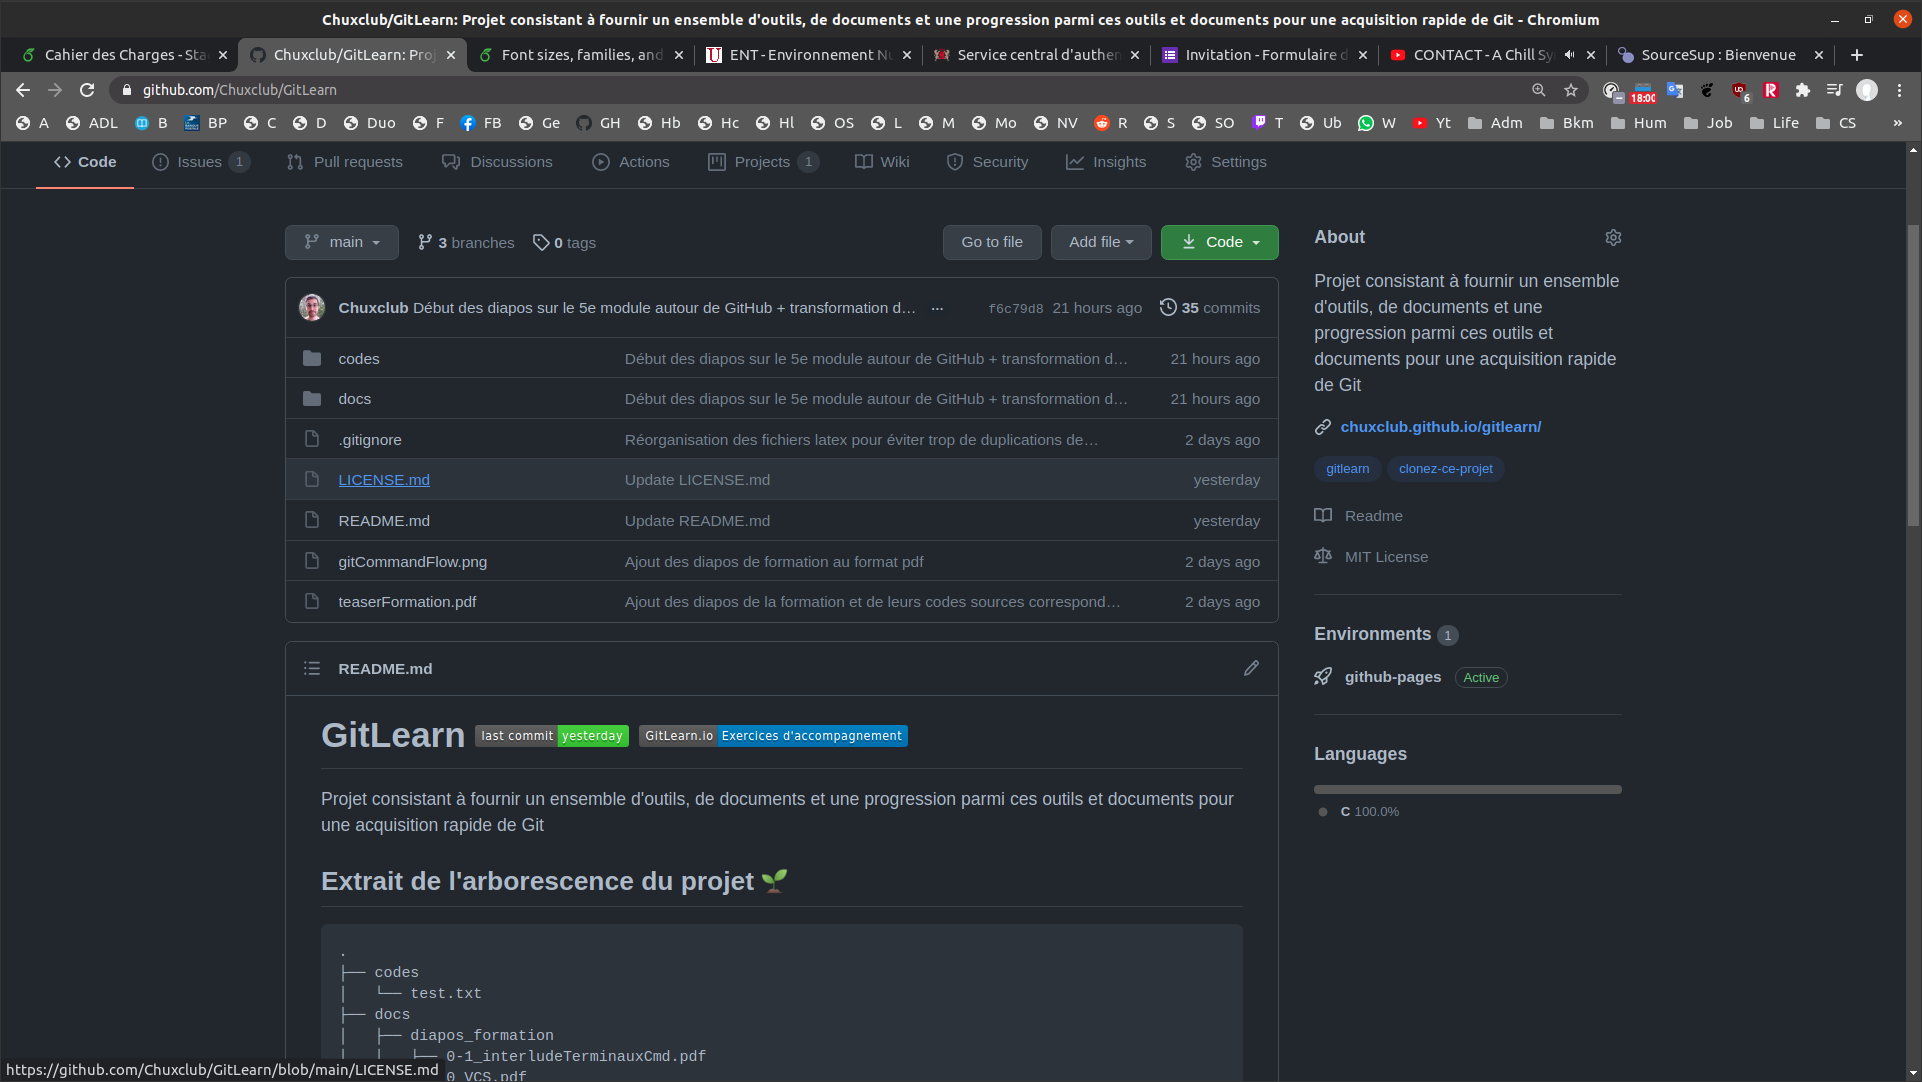
\includegraphics[scale=0.15]{github_fichiersSpeciaux.png}
\end{center}
\end{frame}


\begin{frame}{Le fichier LICENSE}
À l'instar du README le fichier LICENSE est analysé par un robot pour afficher cette licence dans la page d'accueil de votre projet:
\begin{center}
	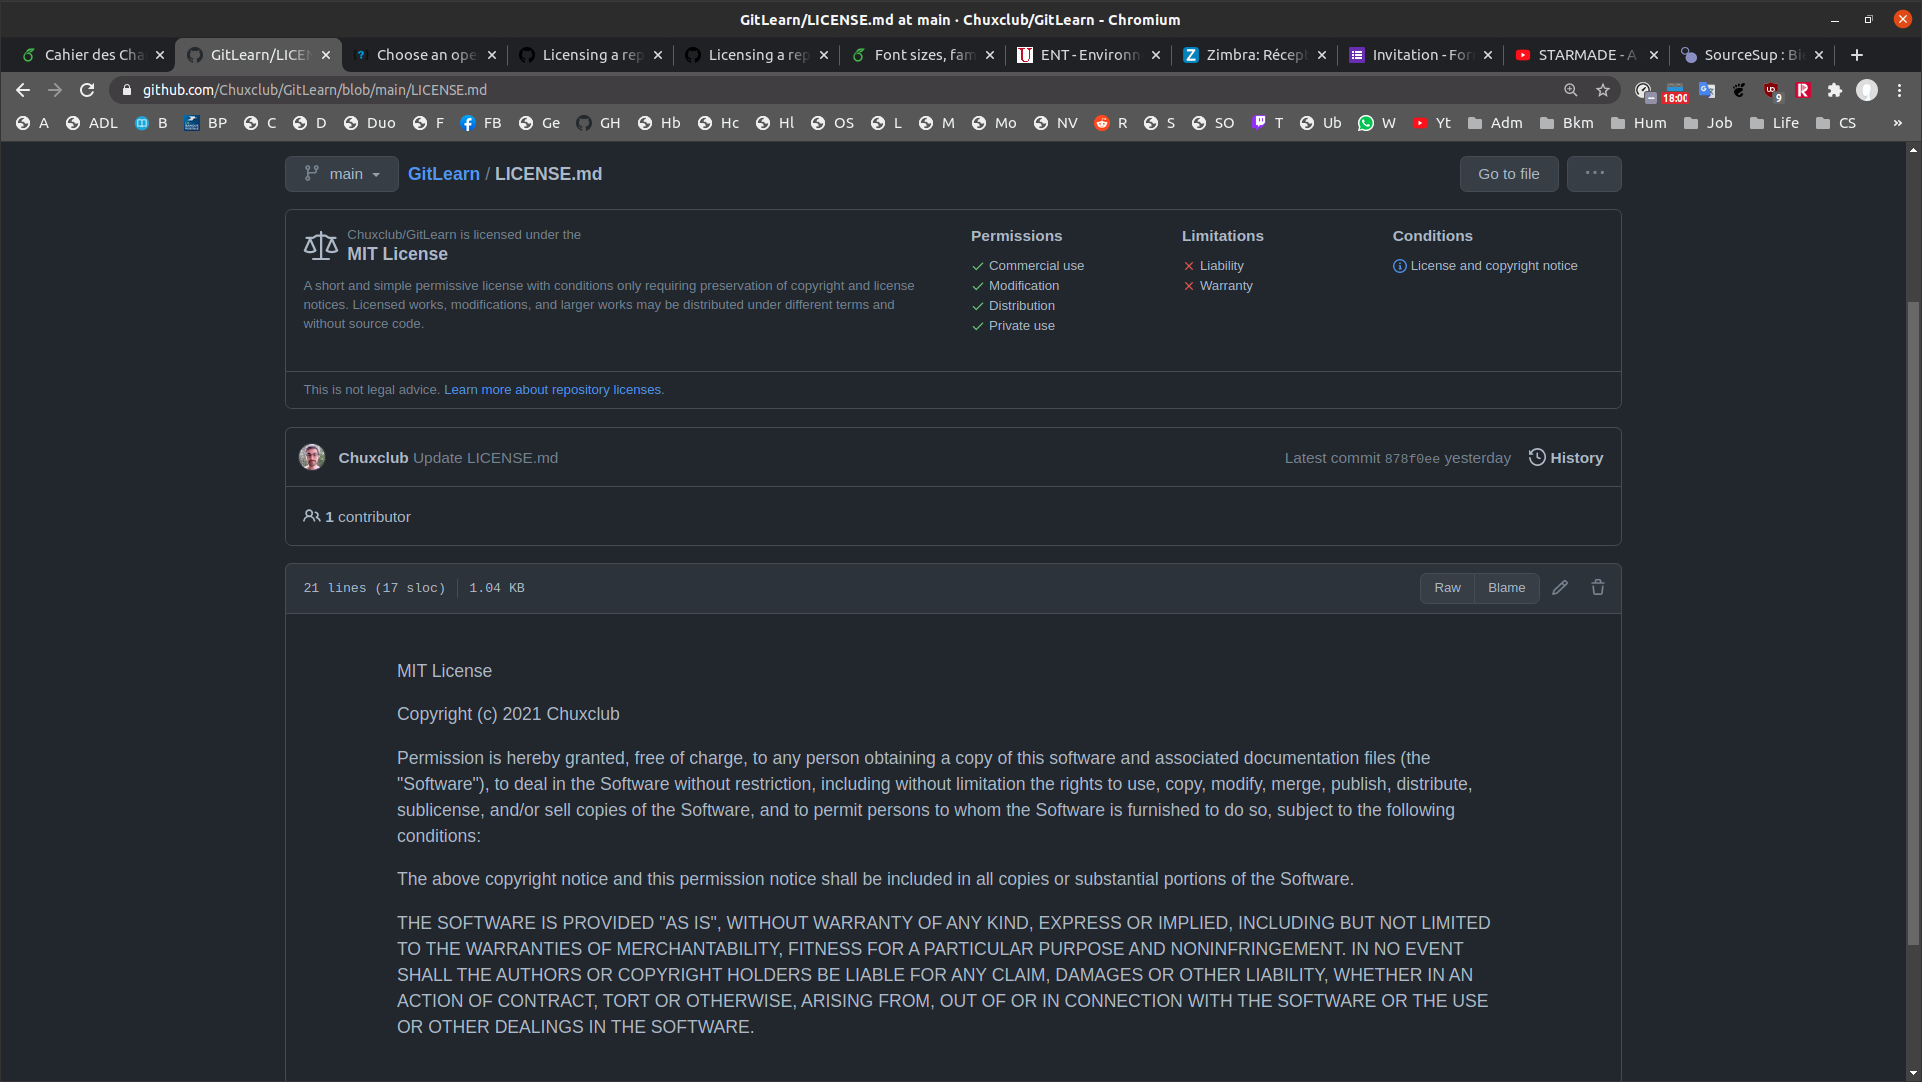
\includegraphics[scale=0.15]{github_license1.png}
\end{center}
\end{frame}


\begin{frame}{Le fichier LICENSE}
Le contenu du fichier LICENSE peut être copié-collé en vous aidant de ce site \url{https://choosealicense.com/}:
\begin{center}
	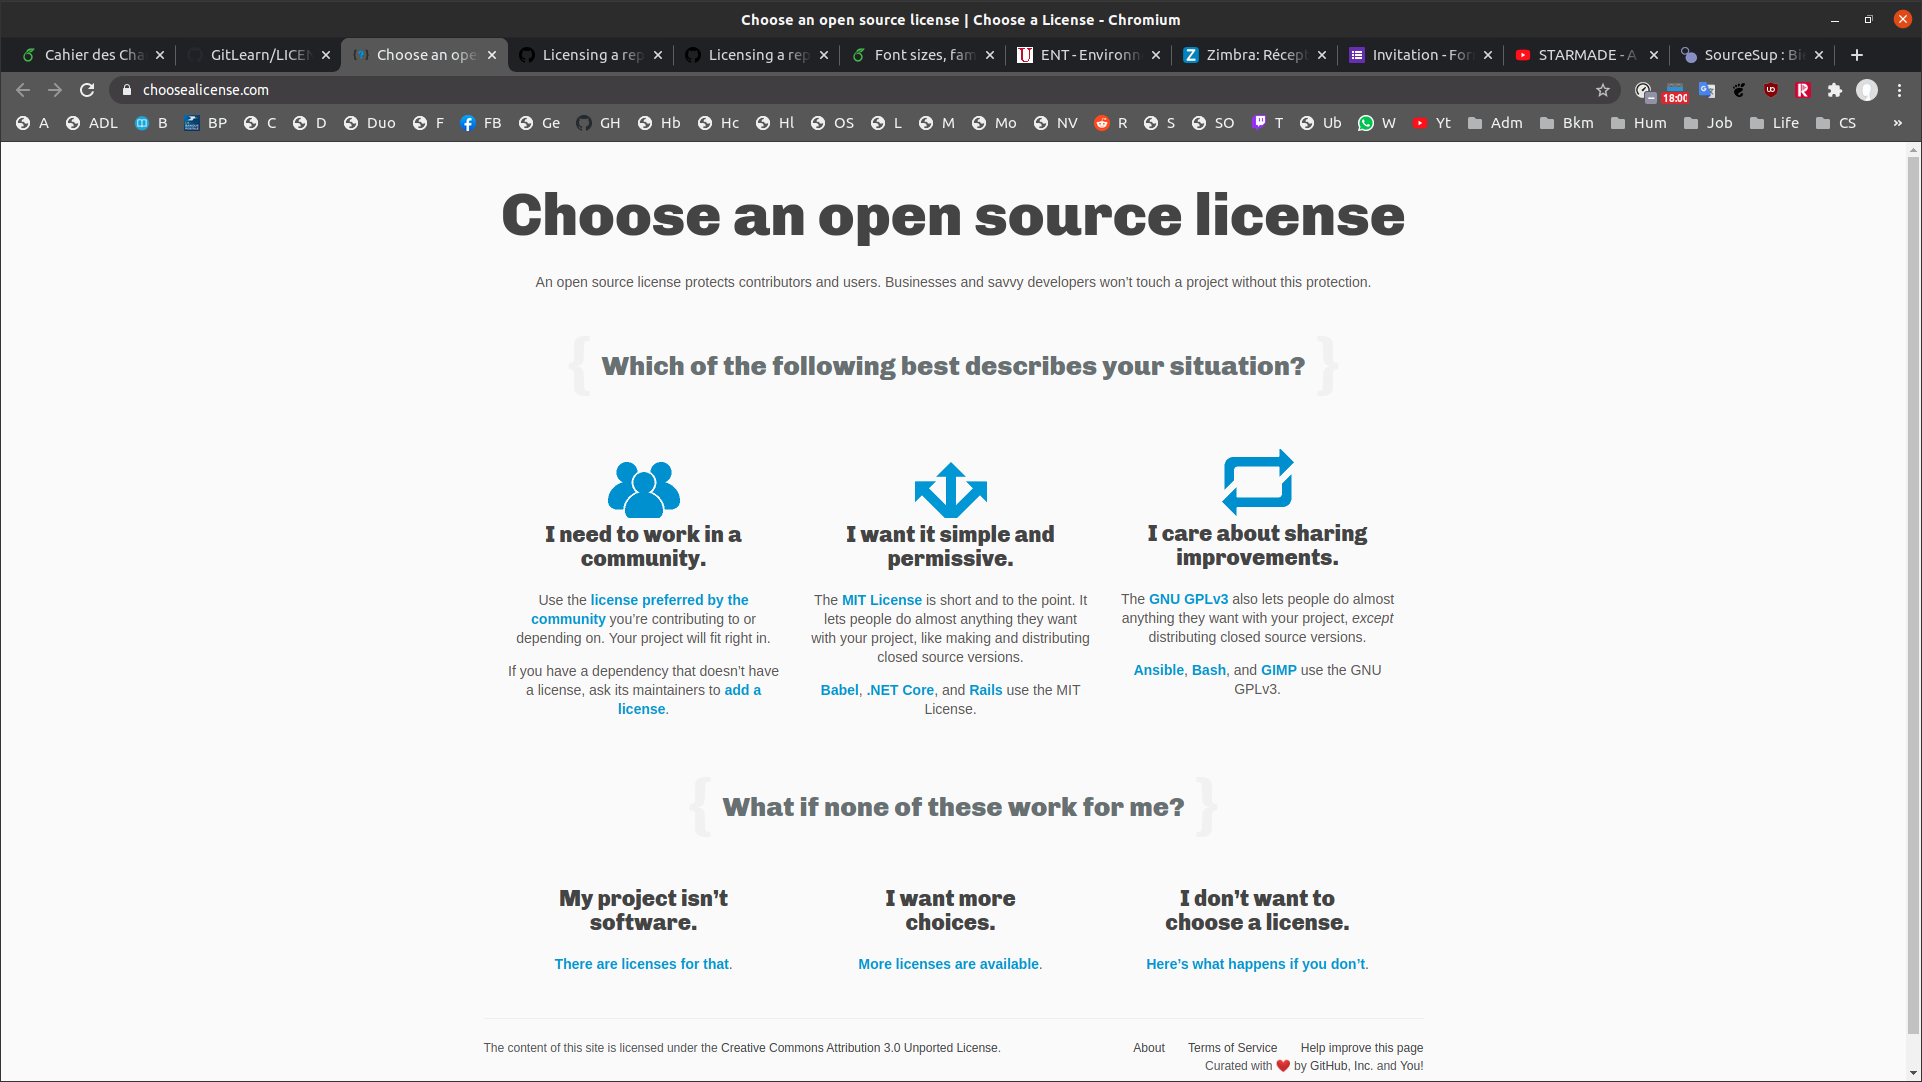
\includegraphics[scale=0.15]{github_license2.png}
\end{center}
\end{frame}


% Subsection:
\subsection{La syntaxe MarkDown}
\begin{frame}{Le guide du MarkDown}

Le MarkDown est un ensemble de petits codes syntaxiques qui permettent de formatter automatiquement un document. L'ensemble de ces codes tient en une page web \url{https://guides.github.com/features/mastering-markdown/}: 
\begin{center}
	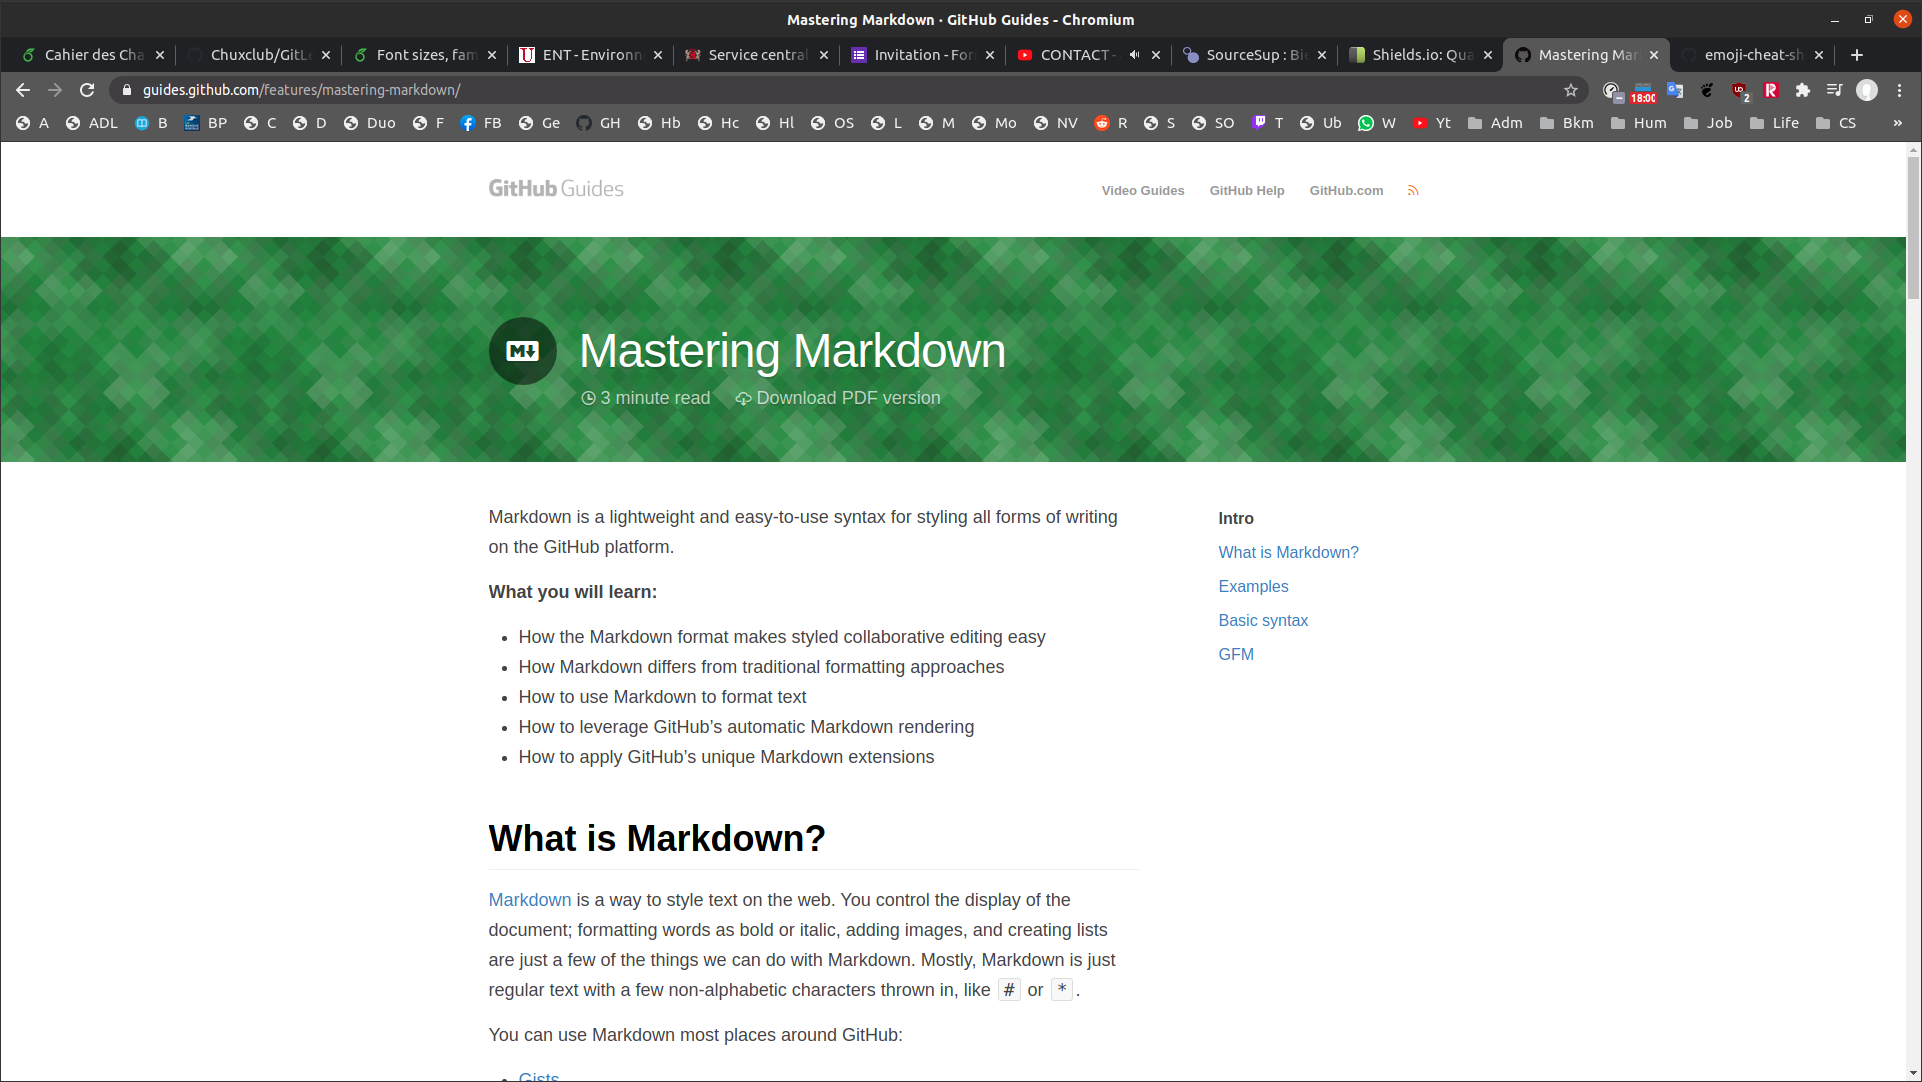
\includegraphics[scale=0.15]{github_markdown.png}
\end{center}
\end{frame}

\begin{frame}{Le guide des emojis en MarkDown}
Il est possible de mettre des emojis dans un README, la page complète vers les codes de ces-derniers se trouve ici \url{https://github.com/ikatyang/emoji-cheat-sheet/blob/master/README.md}: 
\begin{center}
	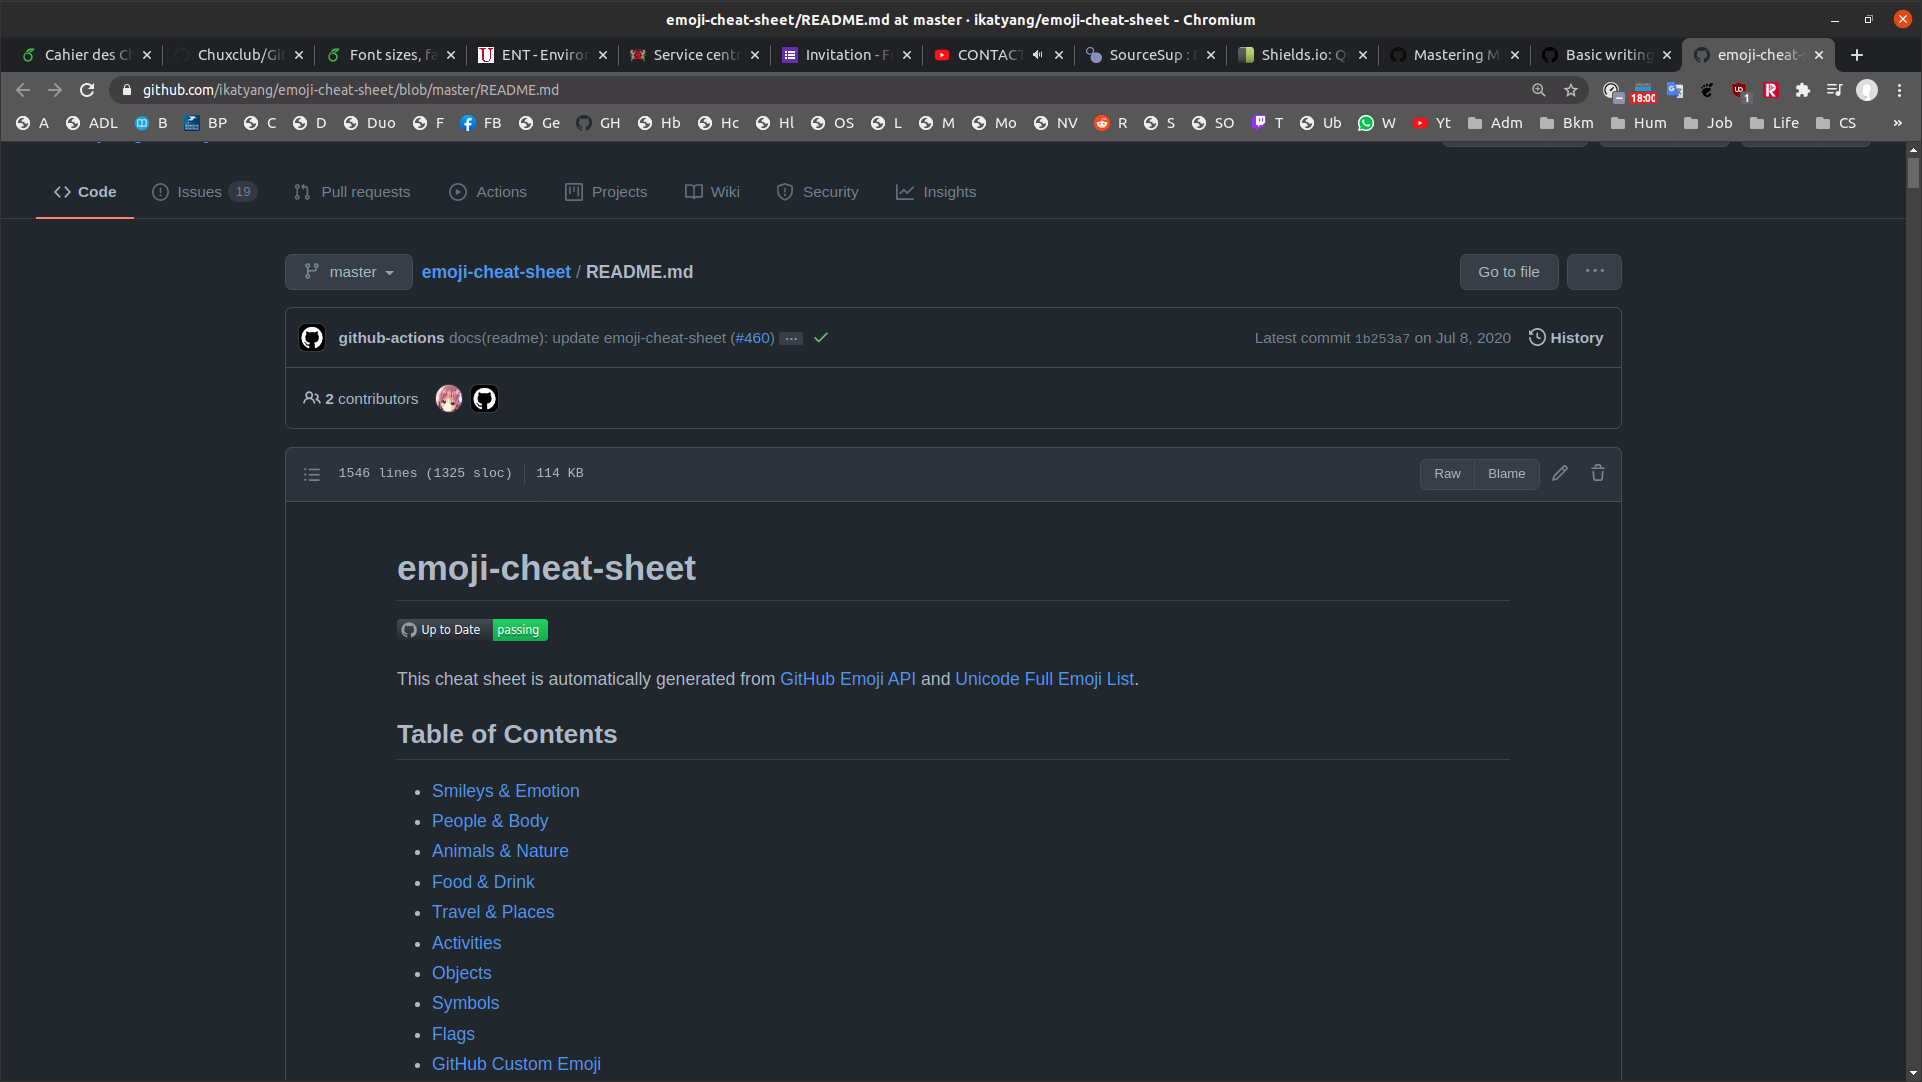
\includegraphics[scale=0.15]{github_emojis.png}
\end{center}
\end{frame}


%% --------------------- %%
%%        SECTION        %%
%% --------------------- %%
\AtBeginSection[]
{
  \begin{frame}
    \frametitle{Table of Contents}
    \tableofcontents[sectionstyle=show/hide,subsectionstyle=show/show/hide]
  \end{frame}
}


\section{Pour aller plus loin avec GitHub}

% Subsection:
\subsection{Le README de son profil}
\begin{frame}{Le dépôt spécial du profil}
Vous pouvez faire apparaître un README sur la page d'accueil de votre profil. Pour ce faire vous devez créer un dépôt dont le nom est celui de votre profil \underline{ET} qui ne contient qu'un README:
\begin{center}
	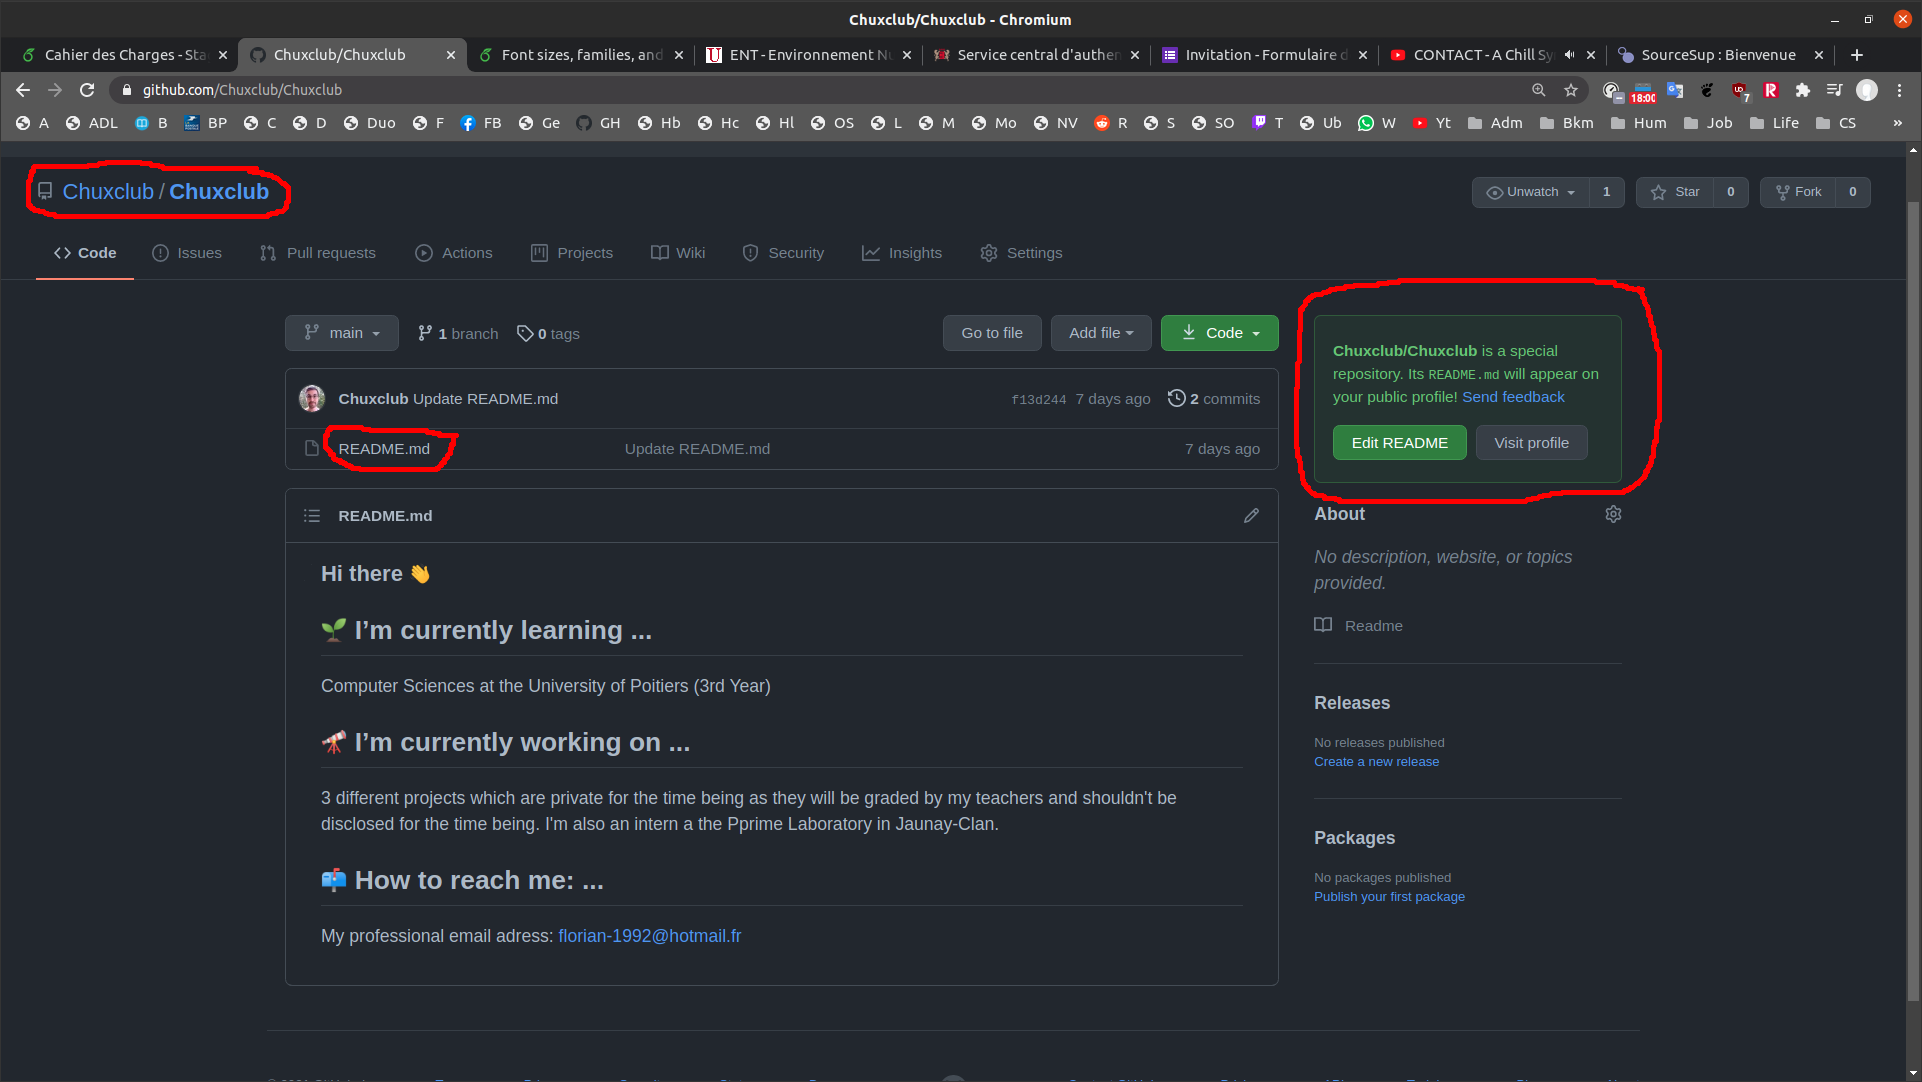
\includegraphics[scale=0.15]{github_depotSpecial_E.png}
\end{center}
\end{frame}


% Subsection:
\subsection{Les Shields en tête du README}
\begin{frame}{Les shields pour des infos en temps réel}
Les shields sont des petits encarts qu'on trouve généralement en tête des README (mais vous pouvez les diposer où vous voulez) et qui ont des fonctionnalités très variables. Le plus fréquemment ils permettent de montrer le dynamisme d'un projet:
\begin{center}
	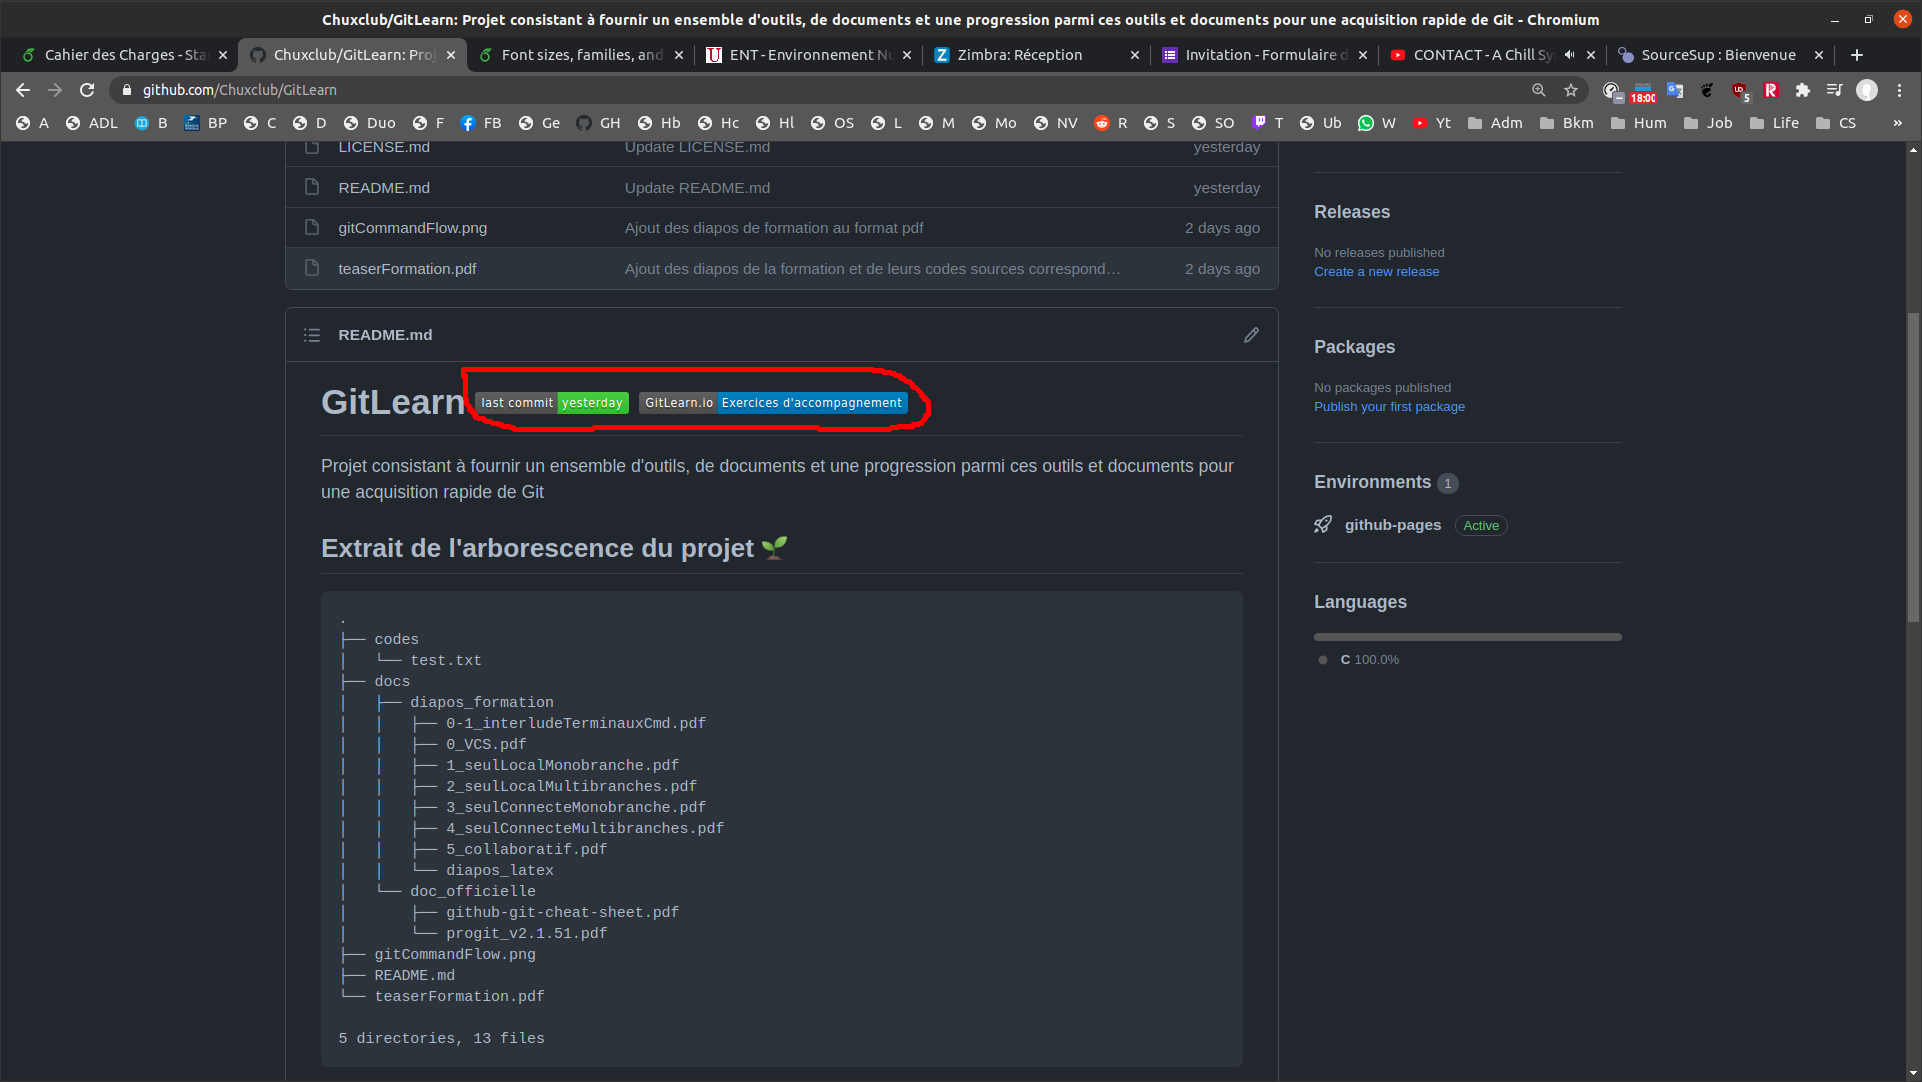
\includegraphics[scale=0.15]{github_shields1_E.png}
\end{center}
\end{frame}

\begin{frame}{Les shields pour des infos en temps réel}
\begin{center}
	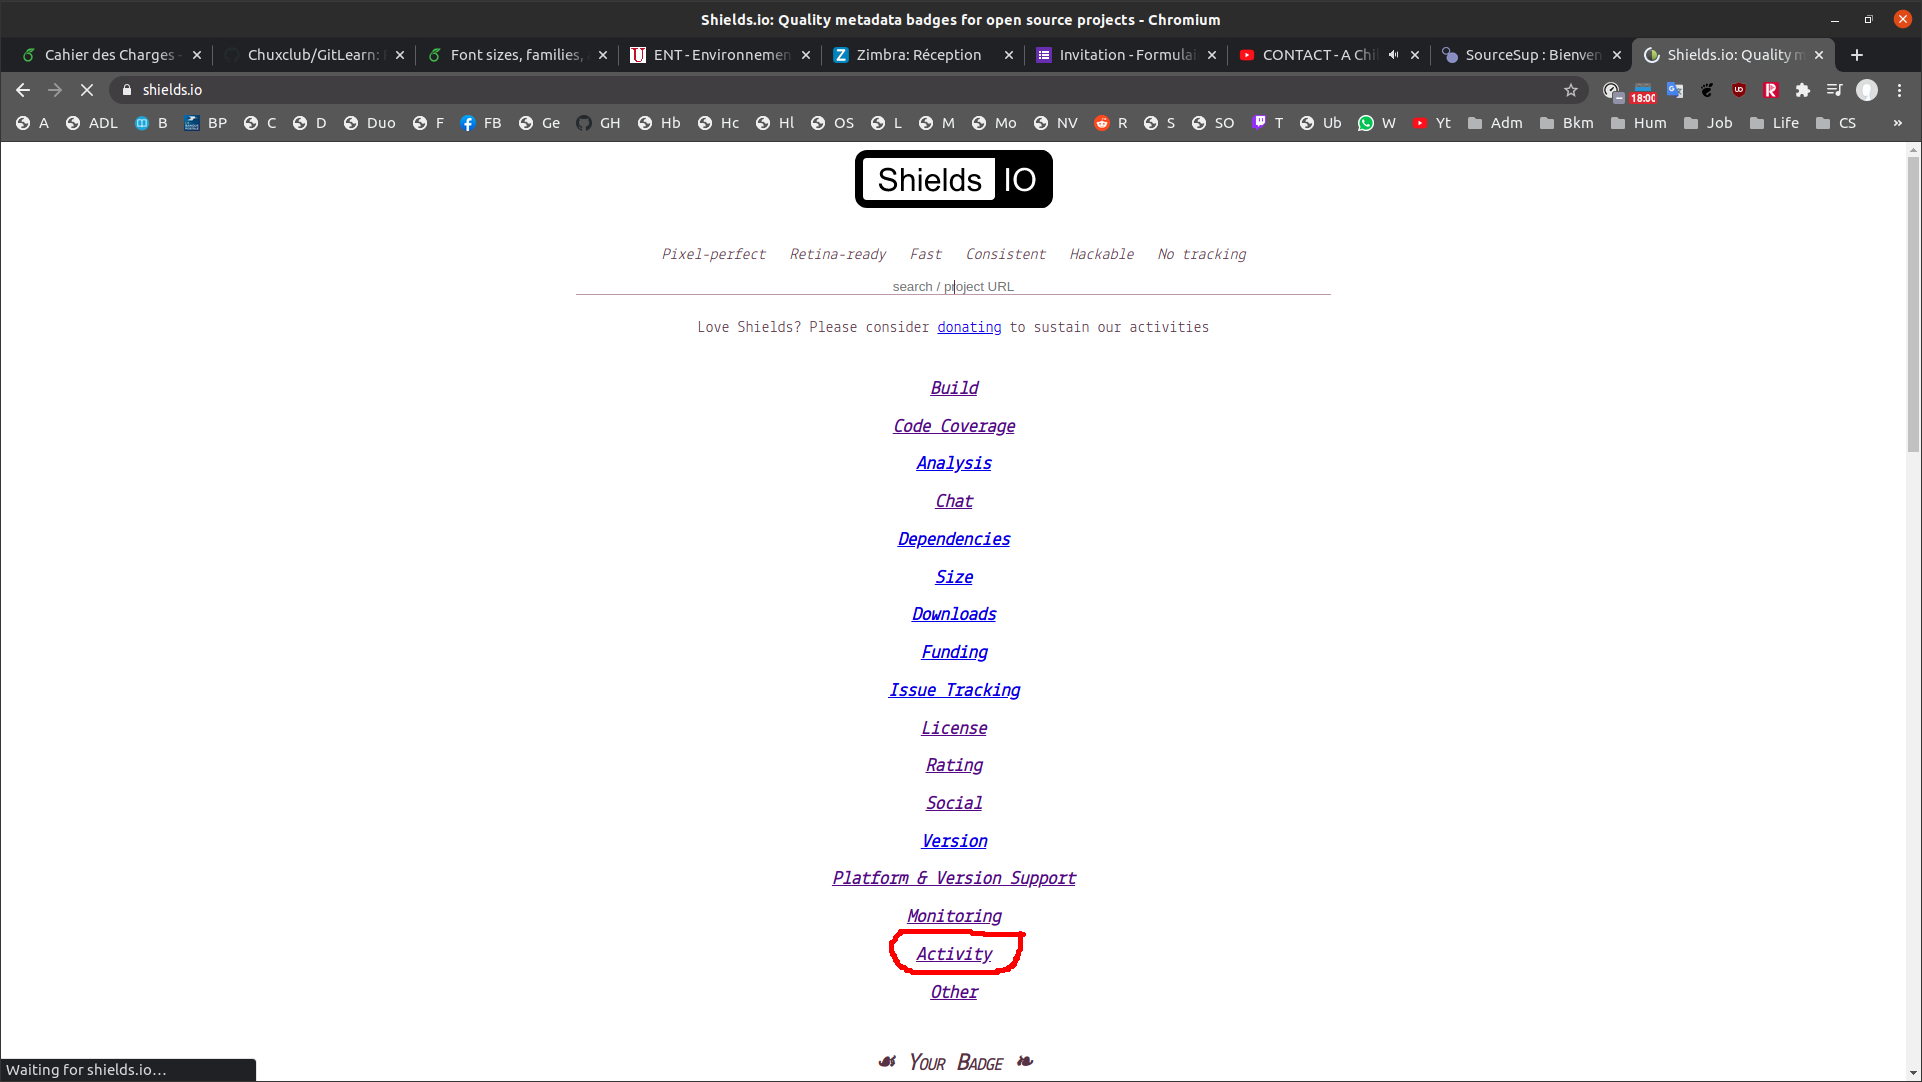
\includegraphics[scale=0.15]{github_shields2_E.png}
\end{center}
\end{frame}

\begin{frame}{Les shields pour des infos en temps réel}
\begin{center}
	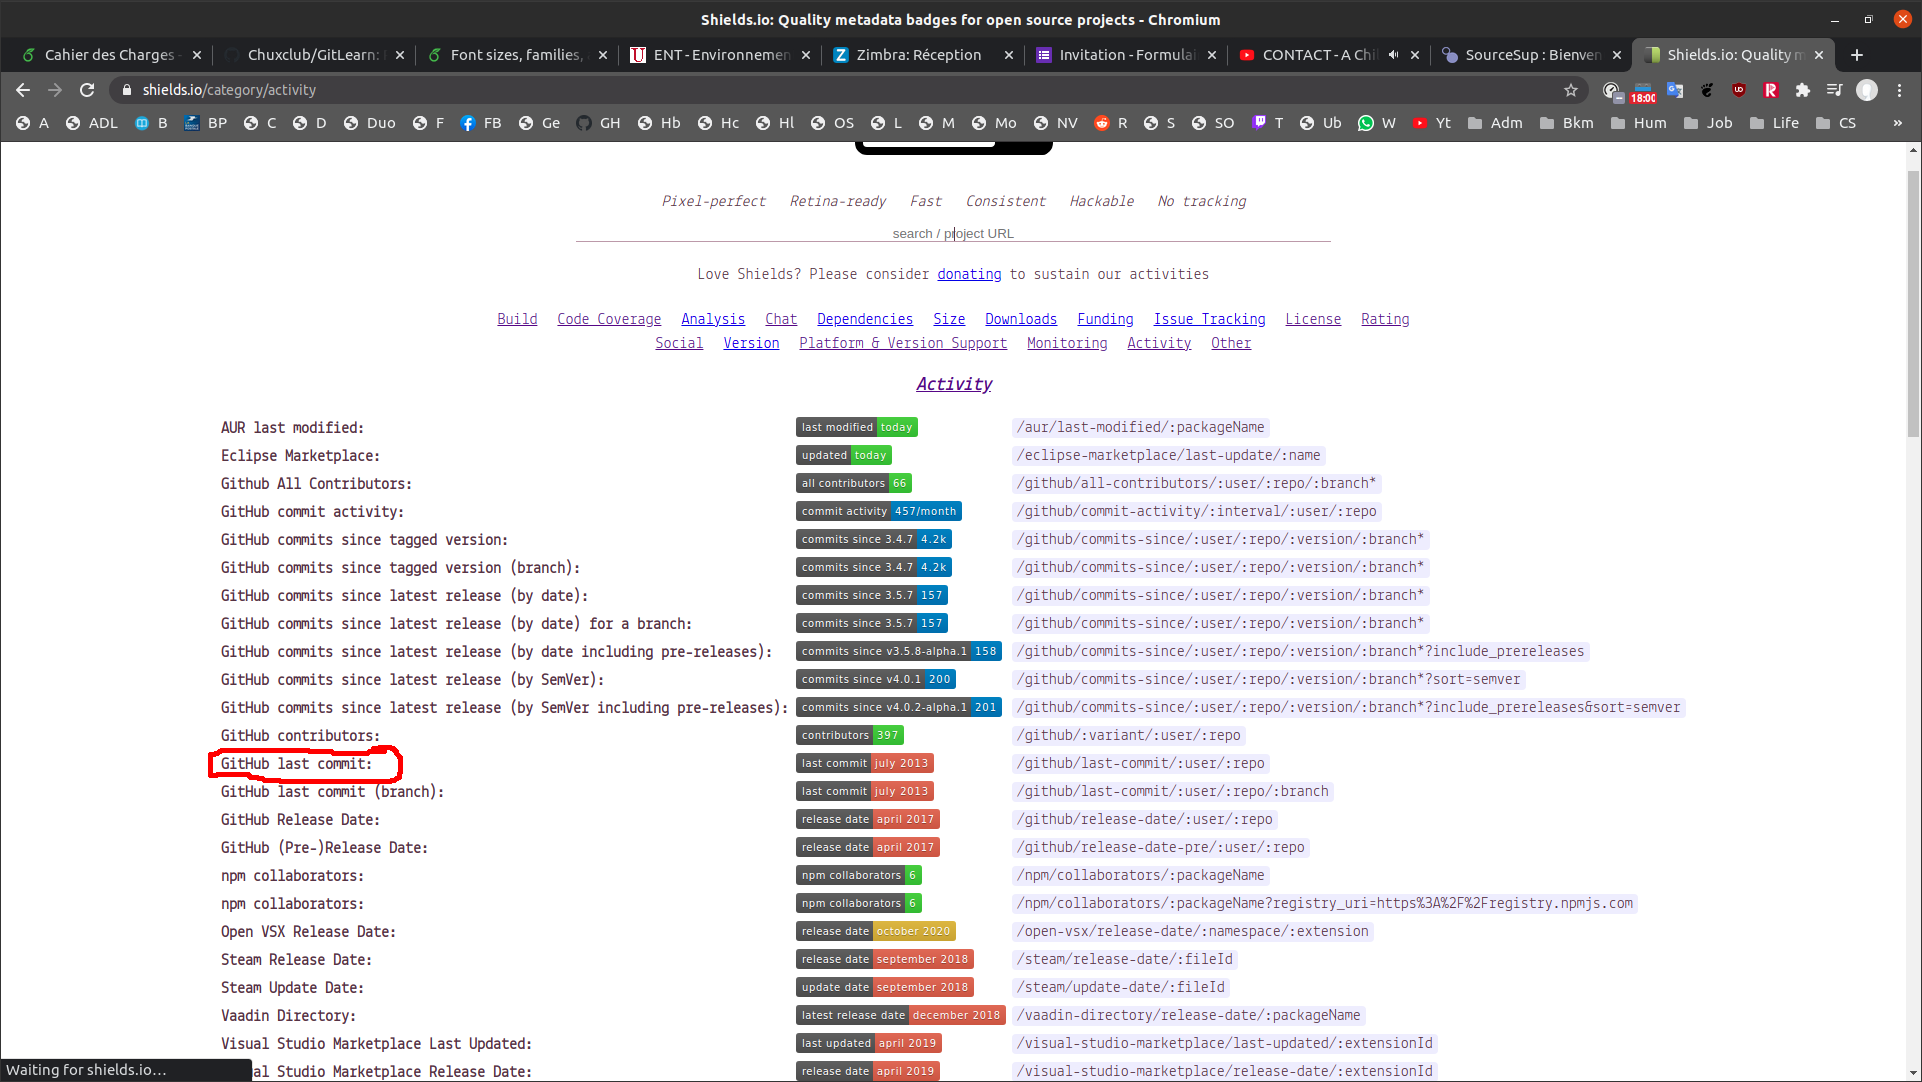
\includegraphics[scale=0.15]{github_shields3_E.png}
\end{center}
\end{frame}

\begin{frame}{Les shields pour des infos en temps réel}
\begin{center}
	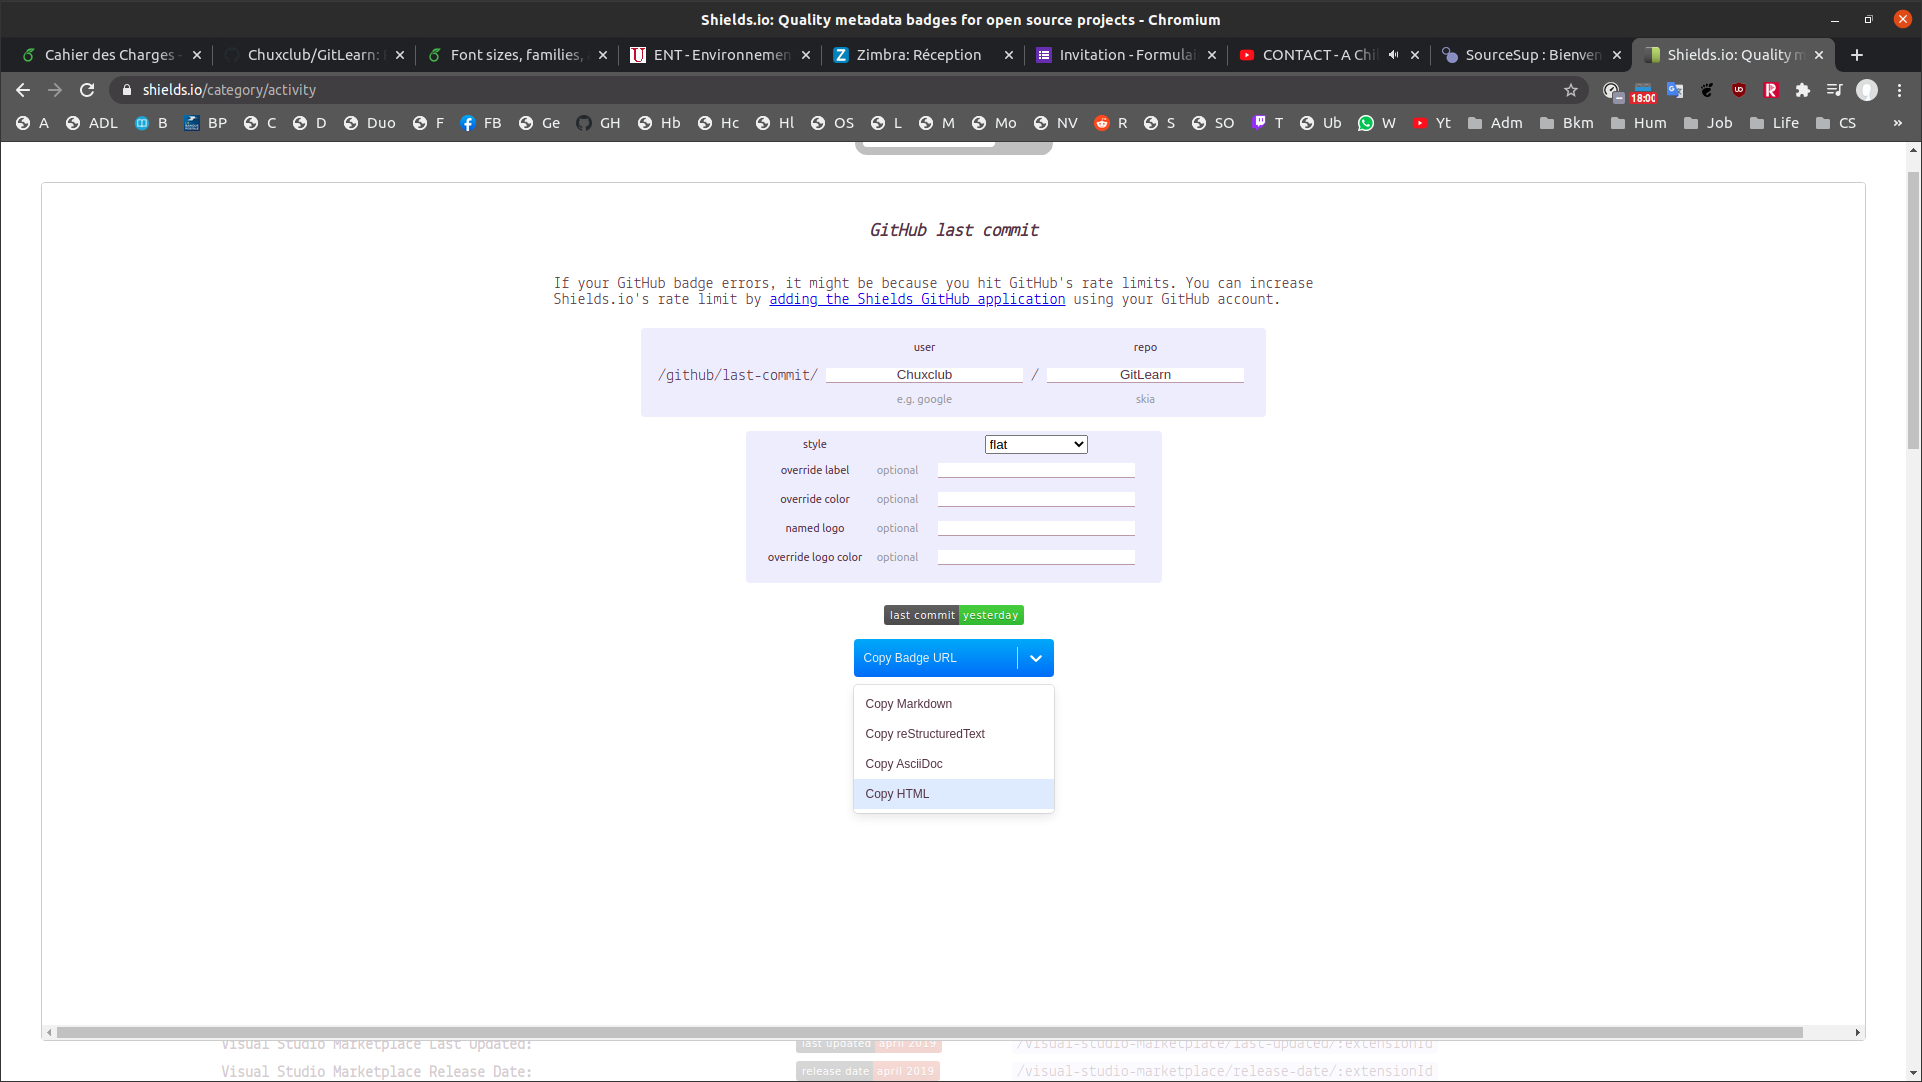
\includegraphics[scale=0.15]{github_shields4.png}
\end{center}
\end{frame}

\begin{frame}{Les shields pour des infos en temps réel}
\begin{center}
	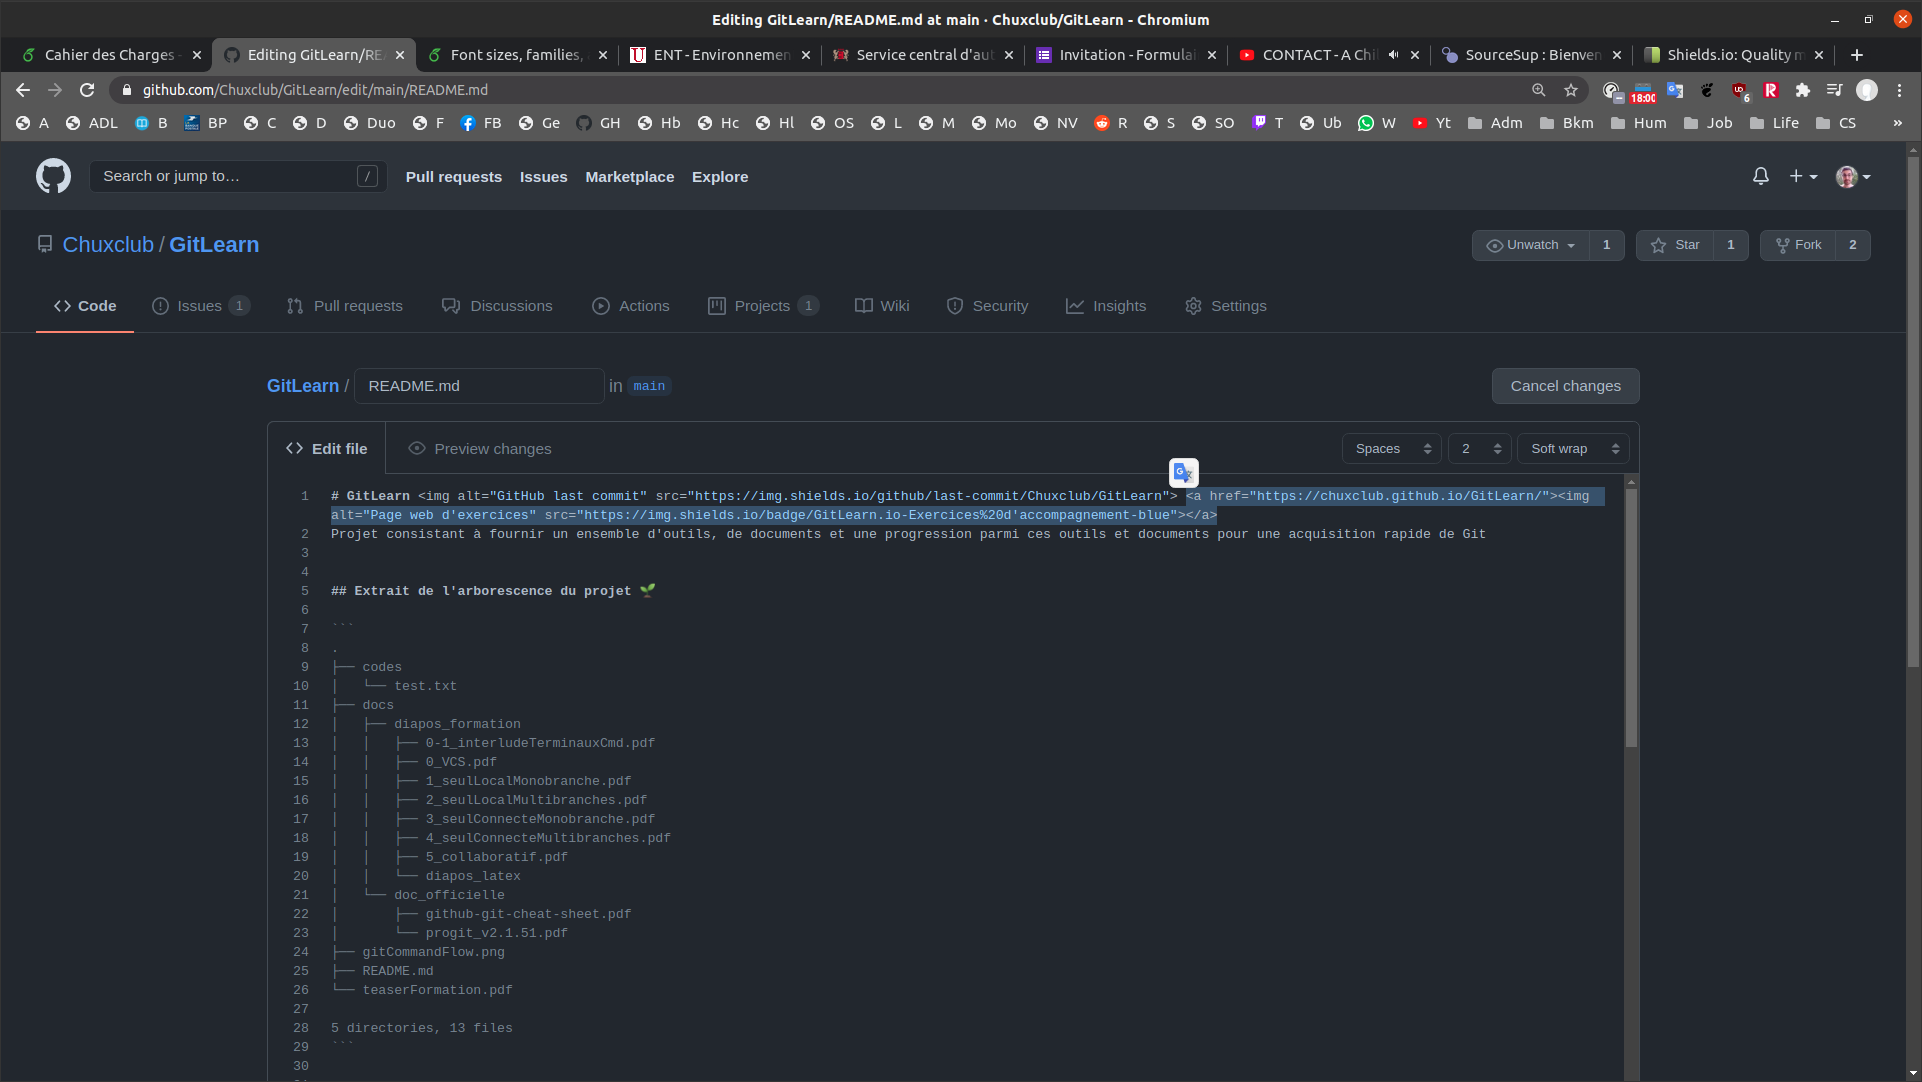
\includegraphics[scale=0.15]{github_shields5.png}
\end{center}
\end{frame}


% Subsection:
\subsection{Les templates de projets}
\begin{frame}{Les templates de projets}
Pour démarrer des projets avec une arborescence standarde et peut-être des fichiers (comme des README?) pré-remplis vous pouvez créer un dépôt publique ou privé:
\begin{center}
	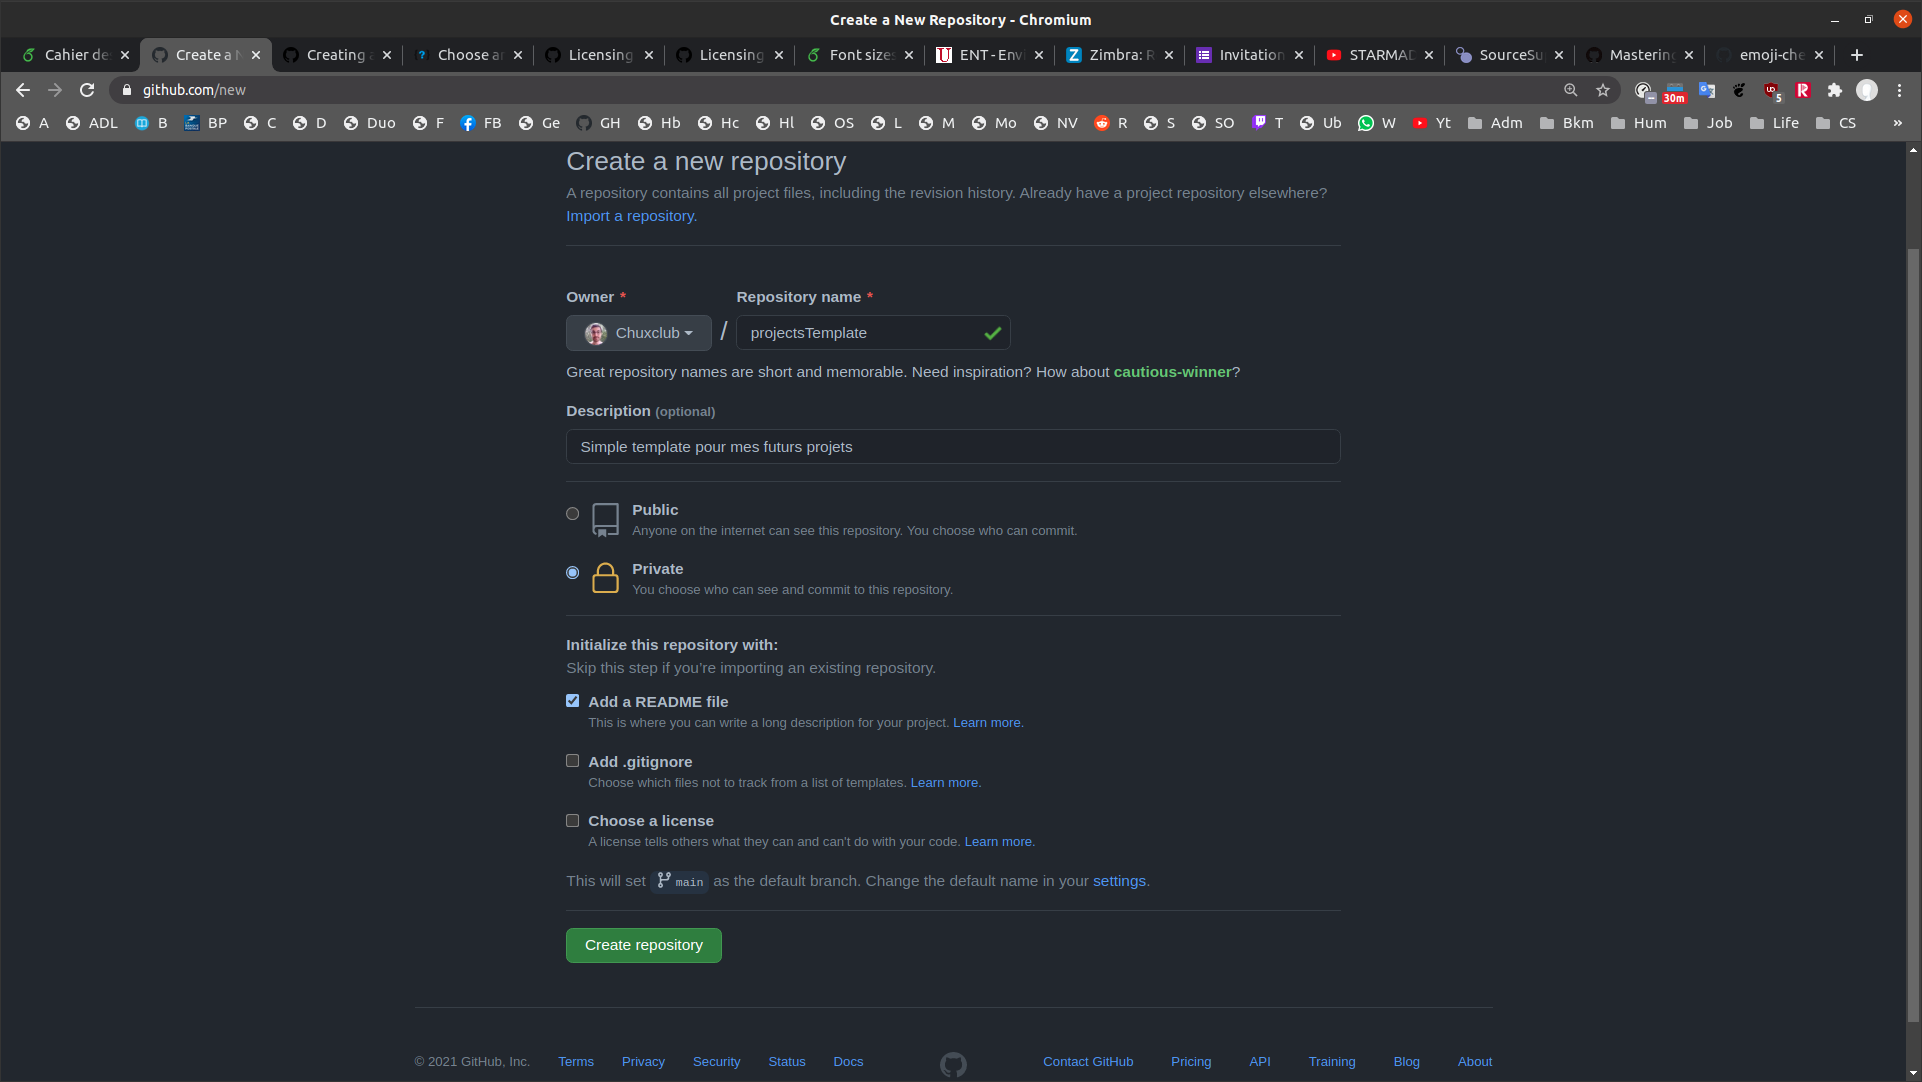
\includegraphics[scale=0.15]{github_repoTemplate1.png}
\end{center}
\end{frame}

\begin{frame}{Les templates de projets}
Puis dans les settings et l'onglet des options du projet vous pouvez indiquer qu'il s'agit d'un template (et non d'un vrai projet!):
\begin{center}
	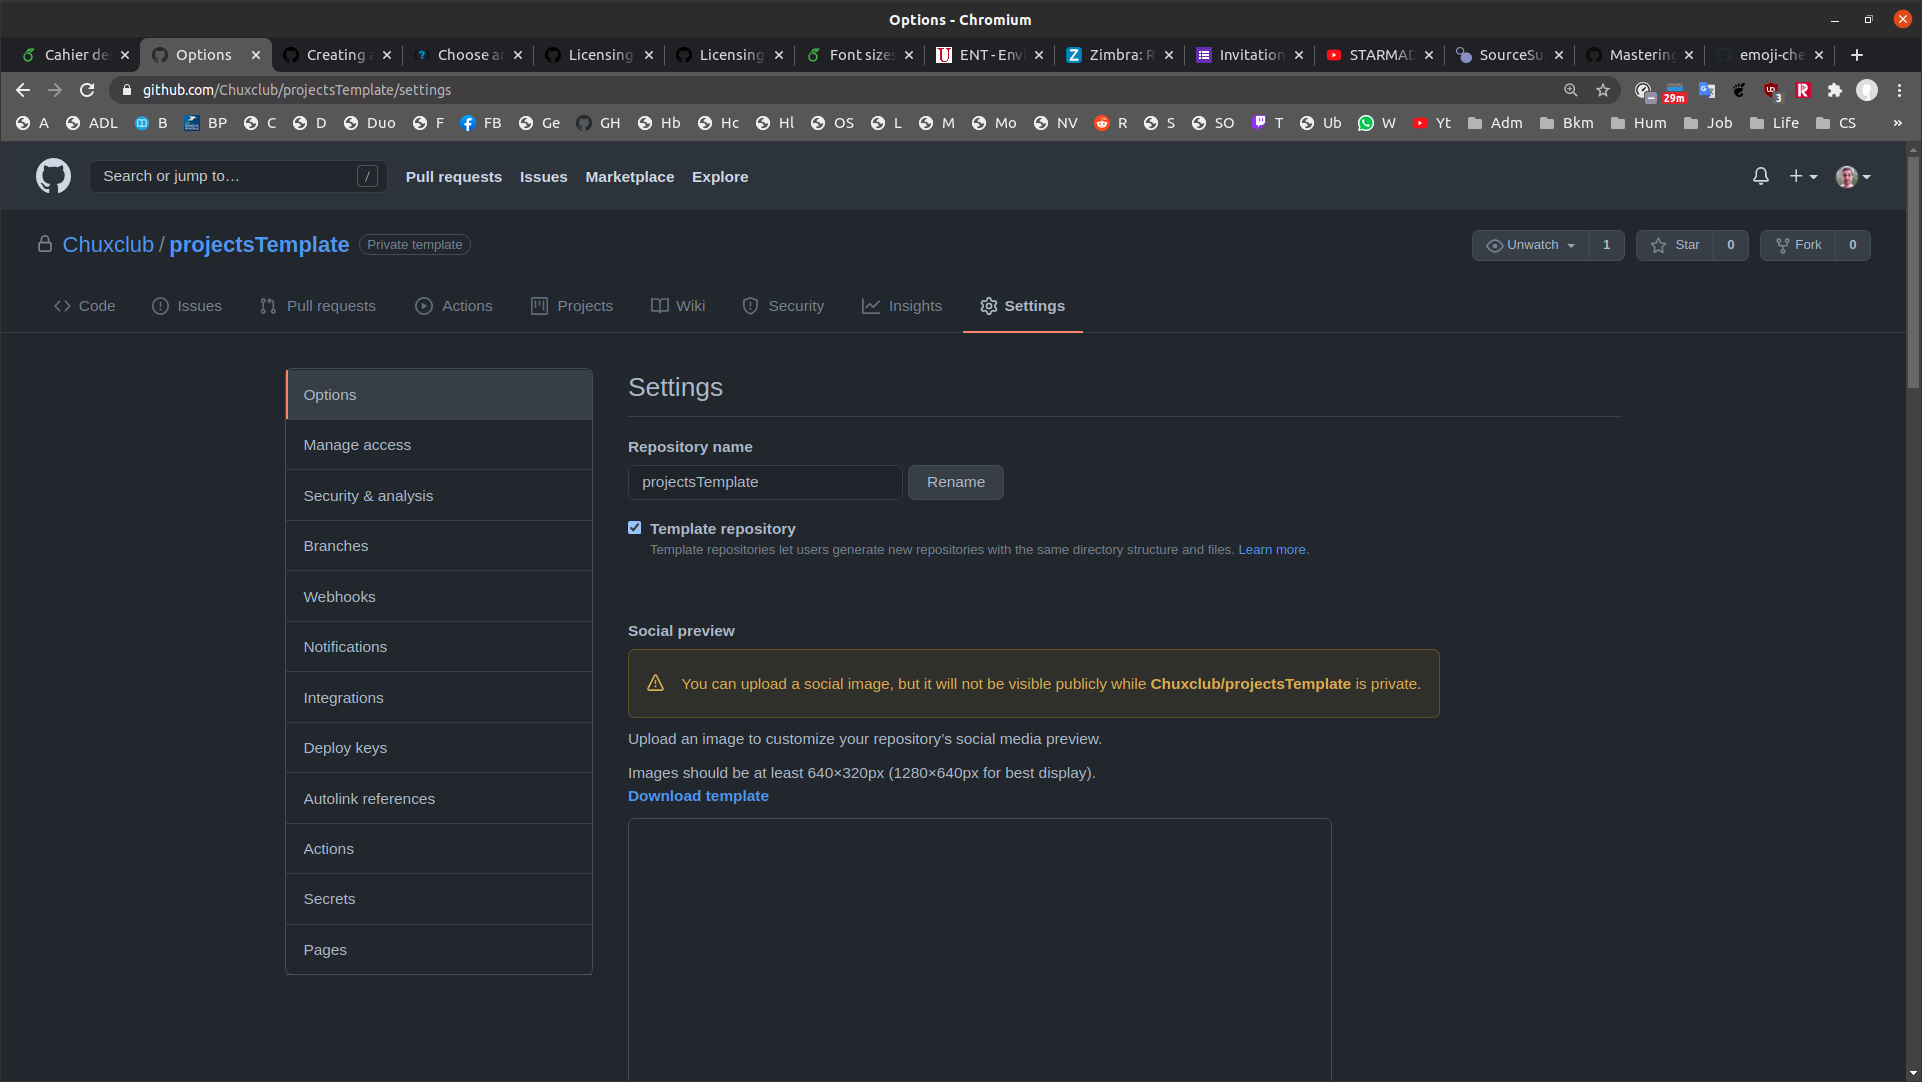
\includegraphics[scale=0.15]{github_repoTemplate2.png}
\end{center}
\end{frame}

\begin{frame}{Les templates de projets}
Il vous suffit alors de cliquer sur "Use this template" pour démarrer un tout projet avec l'arborescence/les fichiers pré-remplis du template en question:
\begin{center}
	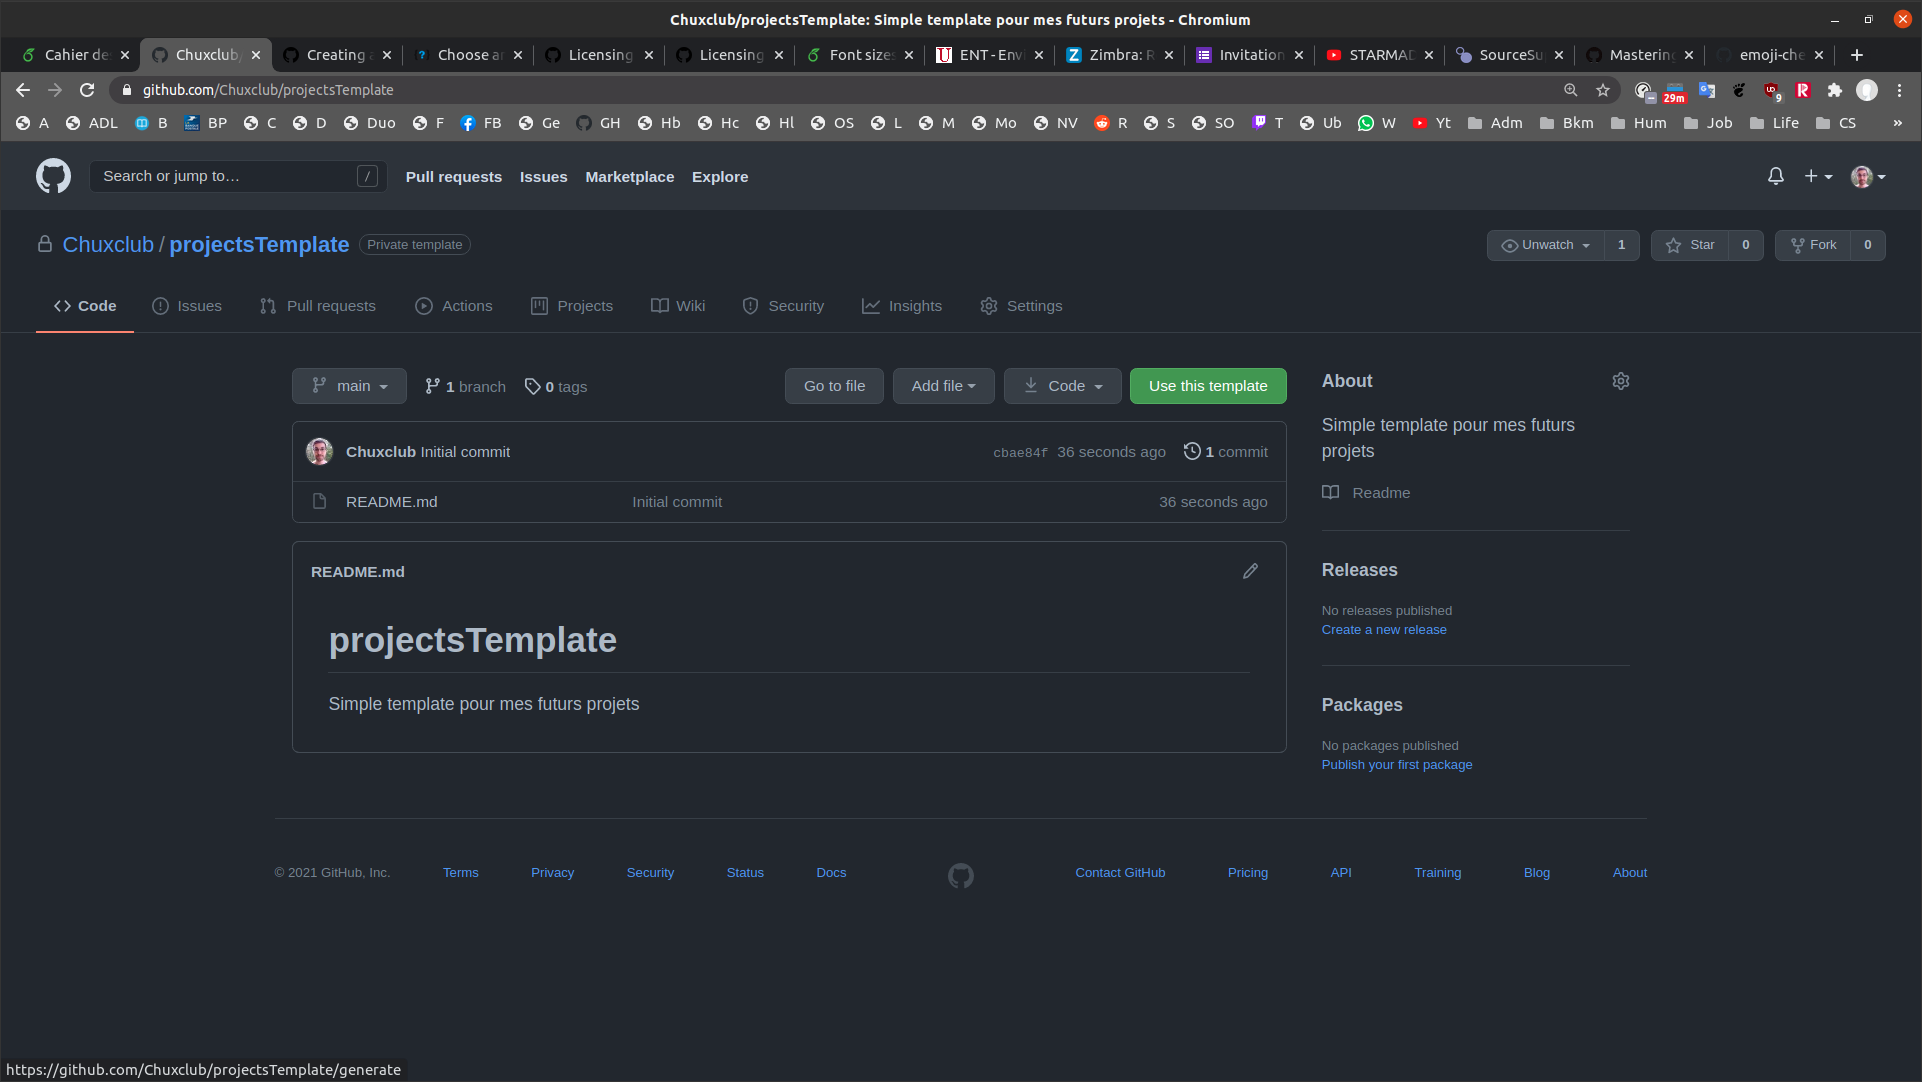
\includegraphics[scale=0.15]{github_repoTemplate3.png}
\end{center}
\end{frame}


% Subsection:
\subsection{Les organisations}
\begin{frame}{Une collaboration à grande échelle avec les organisations}

\end{frame}


% Subsection:
\subsection{Les logiciels avec une API GitHub}
\begin{frame}{Gitter: le Discord des développeurs}

\end{frame}

\begin{frame}{Les applis Android}

\end{frame}


\end{document}